\documentclass[11pt]{article}

% Use wide margins, but not quite so wide as fullpage.sty
\marginparwidth 0.5in
\oddsidemargin 0.25in
\evensidemargin 0.25in
\marginparsep 0.25in
\topmargin 0.25in
\addtolength{\topmargin}{-.75in}
\textwidth 6in
\textheight 8.5in
% That's about enough definitions

\usepackage{fancyvrb,graphicx,float,indentfirst}

\begin{document}

\author{
  Anderson, Anna\      \qquad\texttt{anna.anderson@colorado.edu}
  \and
  Cuthbertson, Sam\      \qquad\texttt{samuel.cuthbertson@colorado.edu}
  }

\title{Digital Logic: Project 1}
\maketitle


\newpage
\section{Introduction}

Beginning to understand how to code Verilog and start thinking as a digital designer is a large task. The point of this lab was to begin to gain a familiarity with a broad range of Verilog commands, explore the differences between procedural versus continuous assignment, and learn about good practices when it comes to digital design. Some of these practices included starting well. Constructing detailed block diagrams from the very beginning not only helped our personal understanding or brought to light conceptual places we were struggling, but it implicitly outlined the code that we ended up writing. This helped the development process.

Beginning at Figure \ref{fig:topdrawn}, we began working through the lab conceptually. Though this changed slightly after we began coding, it is still largely accurate. Our first seven switches go into the specific modules that we made: arithmetic, logical, and comparison. These switches enabled us to perform each of the functions that the individual modules required. However, switches 8 and 9 determine which state displays on the seven segment display and LED. For example, in comparison, these switches chose between equal to, greater than, less than, and max.

\begin{figure}[H]
    \centering
    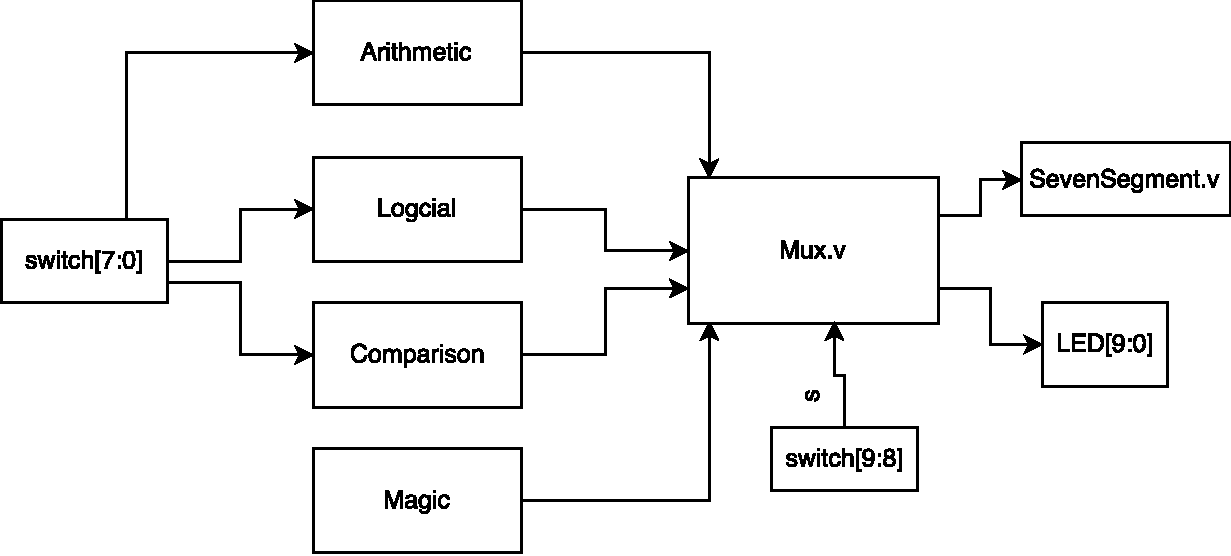
\includegraphics[clip, width=0.8\textwidth]{Top_BD.pdf}
    \caption{Block Diagram of Top Module}
    \label{fig:topdrawn}
\end{figure}


\section{Procedures}
\subsection{Conceptual to Generated}
\subsubsection{Logical and General Verilog Design}
We began with the logical module (See Figure \ref{fig:logicaldrawn}). Drawing this module out was very straight forward which is why, after drawing the rest of the modules, we began by coding this one first. This proved to be a good choice as it brought to light some important conceptual ideas that propagated through to the other modules. For one, figuring out how to pass information out of the module and have it received by other modules turned out to be a sticking point. Realizing that we could and should treat anything outside of the module as though we were writing the module as a black box is what ended up making the development process much easier. Pass in 8 bits of information. Pass out 8 bits of information, or whatever was necessary for the particular module. This simplified and streamlined our process a great deal, and is very apparent when viewing our code in the form of a block diagram in Figure \ref{fig:logicalgen}.

\subsubsection{Comparison, Arithmetic and Block Diagramming Efficiently}
Returning to drawing our block diagrams, we moved on to comparison next (In Figure \ref{fig:comparisondrawn}). We opted for drawing boxed indicating the function that we wanted, as it was advised that Verilog had built in commands for things such as greater than and less than. This allowed us to not over-complicate our process. Thus moving on to arithmetic (In Figure \ref{fig:arithmeticdrawn}), we needed to take into account the LED that should turn on if a carry or remainder was produced. This resulted in a slightly more complicated block diagram.

In this process, it was determined that we should continue to opt for the blocks containing functions such as full adder and subtractor as we realized that the equations given in class were our best bet to constructing this module, and that spending time on block diagramming them in detail would simply be copying down our lecture notes. Additionally, it should be mentioned that we did not build a seven segment display module. As we were thinking through it, we wanted to use case statements in an always statement and did not know how to make a block diagram of it. Under this same reasoning we decided not to make a block diagram of our multiplexer. We still talked about the inputs and outputs that went into it, and being able to physically code it proved to be much more conceptually helpful for us.

\subsubsection{Coding our Diagrams}
After we finished diagramming we moved on to coding in Quartus. From our initial ideas, we did find that some things ended up changing. A significant one ended up being how we processed wanting to use all eight switches under a variable z. Instead of taking z as an input, z was assigned a wire in which the beginning bits were taken from the switches associated with x and the ending ones from those associated with y. This can be seen rather clearly in our generated block diagrams for Logical (Figure \ref{fig:logicalgen}) and for Arithmetic (Figure \ref{fig:arithmeticgen}), as well as our code in \texttt{Logical.v} (lines 7-9) and \texttt{Arithmetic.v} (also lines 7-9).

Our arithmetic module (\texttt{Arithmetic.v}) largely looked as we expected it to. The addition and subtraction modules inside of it this followed the expected format that we went over in class. In the \texttt{fullAdd} module (lines 39-57) we have a \texttt{generate} statement that creates a new instantiation of \texttt{module bAdd} until we have our N-bit adder, where the \texttt{module bAdd} utilizes the equations covered in class. Inside of \texttt{fullAdd}, we have a wire for our carries in order to pass them down the line of \texttt{bAdd} instantiations. This also allows us to return our carry out, as it will be the most significant bit in this wire (line 56).

However, our subtraction modules exploited \texttt{integer i} in it's for loop (line 69). Subtraction proved to be conceptually harder on the front end. However, it's module is shorter. Inside the always block, the difference and borrow wire are iterated over in the \texttt{for} loop on line 75. This is extremely clear as gates in Figure \ref{fig:arithmeticgen}. In this way we still create an N bit subtractor, however it's all contained within the single module.

The multiplication and division modules were much simpler. Each represented a a bit shift in either direction. For the multiplication module, we assigned the carry to the last bit of our input, \texttt{z}, and the first bit of our output to zero, representing the shift (lines 91-92). The rest of output bits were assigned to bits six through zero of our input (line 93). The opposite was done for division. The lowest bit of the input was set to the remainder, while the highest was set to zero (lines 102-103).

The comparison module exactly followed the format that we had outlined in our block diagrams. Less than, greater than, and equal to all represented a keyword for a circuit in Verilog, greatly simplifying the process. Inside comparison, the \texttt{bMax} module was the only one that we ended up needing to modify from the simple box represented in the diagram, as an always statement made much more sense to us after some experience with Verilog. To implement \texttt{bMax}, we made an instantiation of our \texttt{bGreater} (line 48), assigning it's output to a wire. That wire is then referenced within a case statement that allows us to output the value of either x or y, depending on whether x is greater than y. This is much clearer in the genereated block diagram in Figure \ref{fig:comparisongen}

However, Magic was not implemented in the same way that we originally had demonstrated in Figure \ref{fig:topdrawn}. Magic ended up bypassing that selector multiplexer altogether, which we'll cover later.

\subsection{Encoding Schemes}
\subsubsection{Button Modes}
For the buttons to swap between Arithmetic/Comparison/Logical/Magic, we created a \texttt{state} register which would toggle between $0$ and $1$ on \texttt{posedge} of the corresponding button: i.e, \texttt{KEY[0]} would toggle \texttt{state[0]} and \texttt{KEY[1]} would toggle \texttt{state[1]}. For the mode selectors within Arithmetic/Comparison/Logical, we used the direct value from \texttt{SW[9:8]}.

\begin{center}
    \begin{minipage}[t]{0.4\textwidth}
        \begin{center}
            \begin{tabular}{|c|c|}
                \hline
                \multicolumn{2}{|c|}{Top} \\
                \hline
                state & Output \\
                \hline
                $00$ & Arithmetic \\
                $01$ & Logical \\
                $10$ & Comparison \\
                $11$ & Magic \\
                \hline
            \end{tabular}
        \end{center}
    \end{minipage}
    \begin{minipage}[t]{0.4\textwidth}
        \begin{center}
            \begin{tabular}{|c|c|}
                \hline
                \multicolumn{2}{|c|}{Arithmetic} \\
                \hline
                selector & Output \\
                \hline
                $00$ & Addition(x,y) \\
                $01$ & Subtraction(x,y) \\
                $10$ & Multiply by 2(z) \\
                $11$ & Divide by 2(z) \\
                \hline
            \end{tabular}
        \end{center}
    \end{minipage}
\end{center}

\begin{center}
    \begin{minipage}[t]{0.4\textwidth}
        \begin{center}
            \begin{tabular}{|c|c|}
                \hline
                \multicolumn{2}{|c|}{Comparison} \\
                \hline
                selector & Output \\
                \hline
                $00$ & Equal(x,y) \\
                $01$ & XGreater(x,y) \\
                $10$ & XLess(x,y) \\
                $11$ & Max(x,y) \\
                \hline
            \end{tabular}
        \end{center}
    \end{minipage}
    \begin{minipage}[t]{0.4\textwidth}
        \begin{center}
            \begin{tabular}{|c|c|}
                \hline
                \multicolumn{2}{|c|}{Logical} \\
                \hline
                selector & Output \\
                \hline
                $00$ & And(x,y) \\
                $01$ & Or(x,y) \\
                $10$ & xOr(x,y) \\
                $11$ & Not(z) \\
                \hline
            \end{tabular}
        \end{center}
    \end{minipage}
\end{center}

\subsubsection{Wire Arrangements in Top.v}

For the output from each of Arithmetic/Comparison/Logical, we expected the ordering shown below.
\begin{center}
    \begin{tabular}{|c|c|c|c|c|c|c|c|c|c|}
        \hline
        Bit Count & 0 & 1 & 2 & 3 & 4 & 5 & 6 & 7 & 8 \\
        \hline
        Output Value & \multicolumn{4}{|c|}{Lower 7seg} & \multicolumn{4}{|c|}{Higher 7seg} & LED9 \\
        \hline
    \end{tabular}
\end{center}

We also hard coded the input from magic to our Mux to be $1'b0$, which would set both seven segment displays to 0 for the magic mode. Additionally, the output from the magic module was sent to the LEDs only when our \texttt{state} register was $11$.

Finally, our \texttt{state} register is also used as input to our \texttt{SevenSegmentMode} module in order to display the current mode we are in, as one of A, L, C or M for magic.

\section{Results}
\subsection{Output Pictures}
\begin{figure}[H]
    \centering
    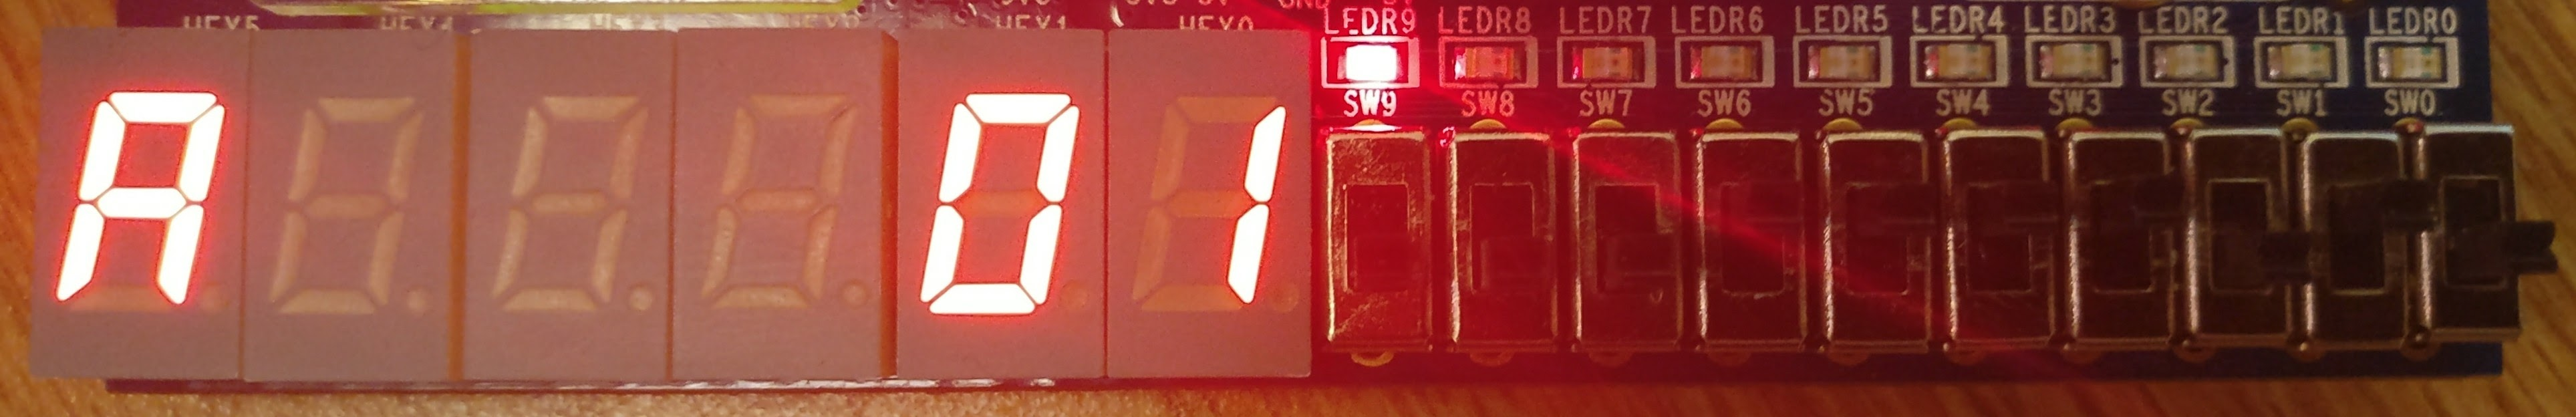
\includegraphics[width=0.8\textwidth]{Ar1}
    \caption{Our output for adding 0xA and 0x7, showing that it is 0x11}
\end{figure}
\begin{figure}[H]
    \centering
    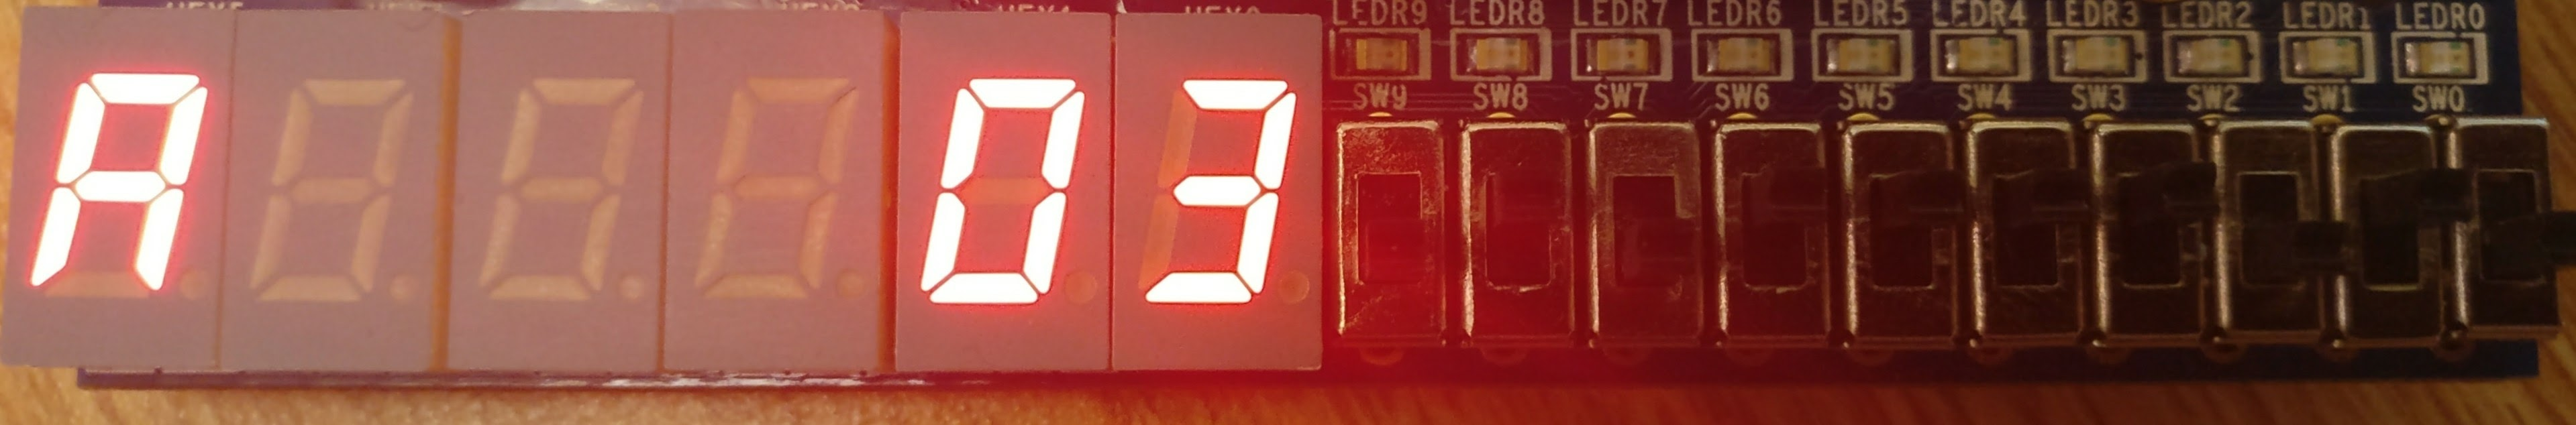
\includegraphics[width=0.8\textwidth]{Ar2}
    \caption{Our output for subtracting 0x7 from 0xA, showing that it is 0x3}
\end{figure}
\begin{figure}[H]
    \centering
    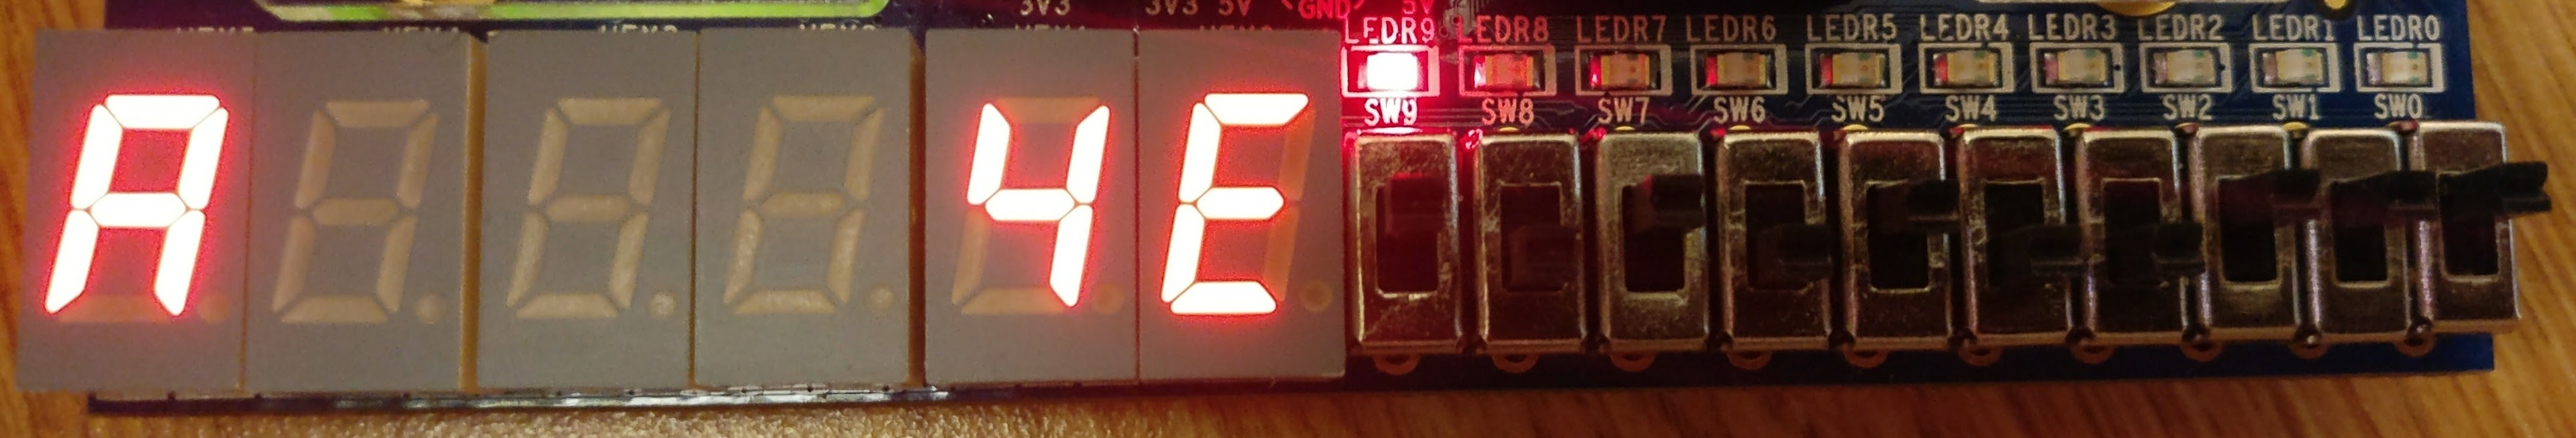
\includegraphics[width=0.8\textwidth]{Ar3}
    \caption{Our output for multiplying 0xA7 by 2, showing that it is 0x14E}
\end{figure}
\begin{figure}[H]
    \centering
    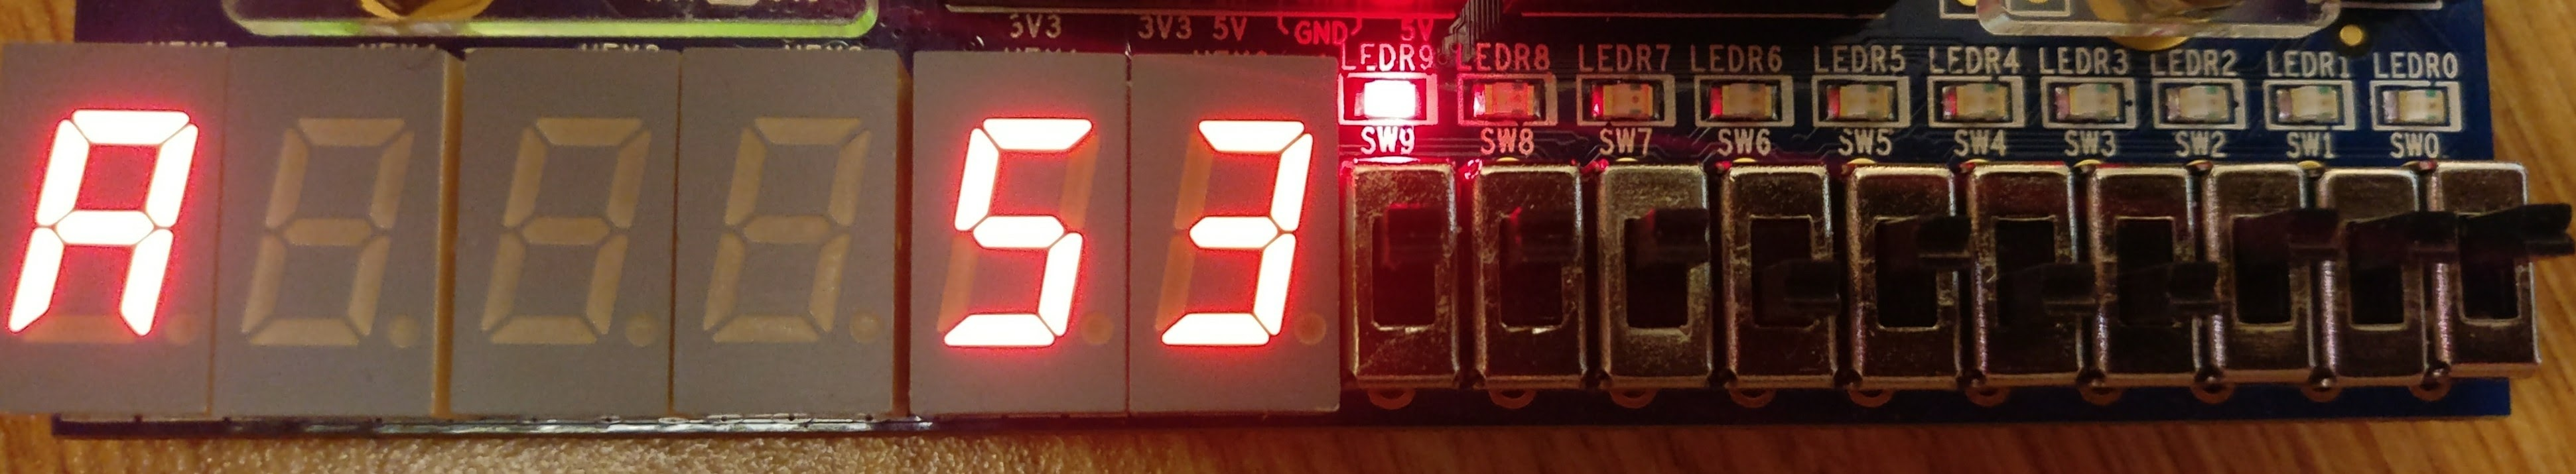
\includegraphics[width=0.8\textwidth]{Ar4}
    \caption{Our output for dividing 0xA7 by 2, showing that it is 0x53 and a half}
\end{figure}

\begin{figure}[H]
    \centering
    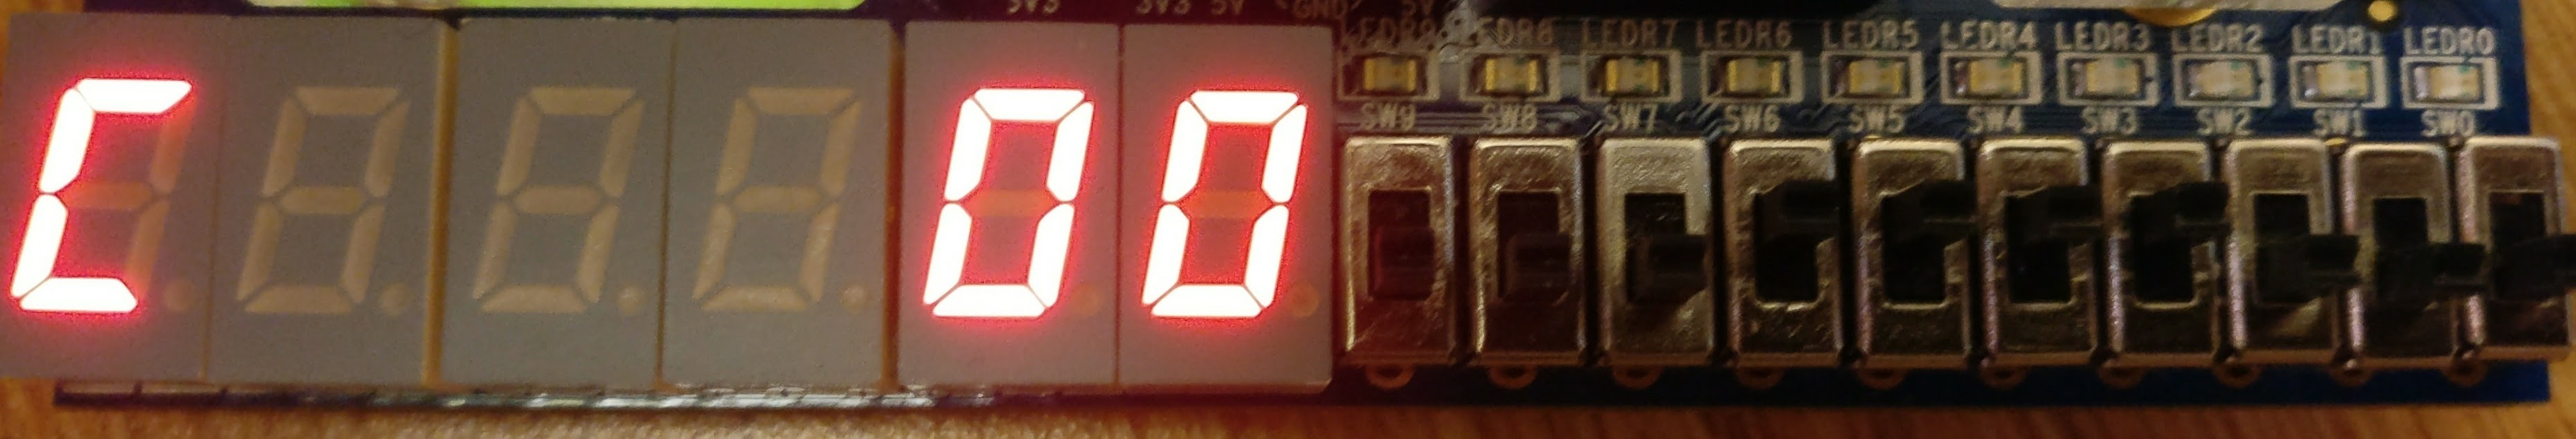
\includegraphics[width=0.8\textwidth]{C1}
    \caption{Our output for seeing if 0x8 and 0x7 are equal, showing that they are not.}
\end{figure}
\begin{figure}[H]
    \centering
    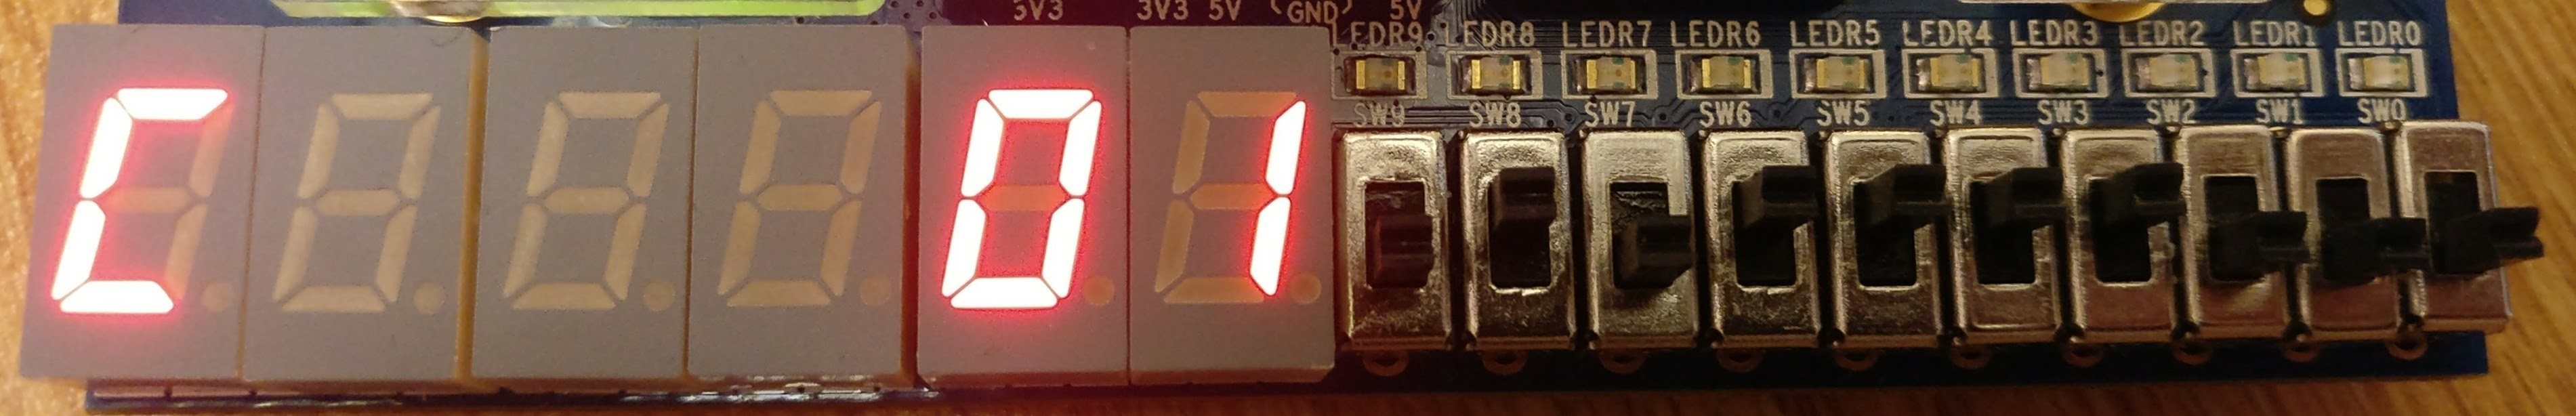
\includegraphics[width=0.8\textwidth]{C2}
    \caption{Our output for seeing if 0x8 is greater than 0x7, showing that it is.}
\end{figure}
\begin{figure}[H]
    \centering
    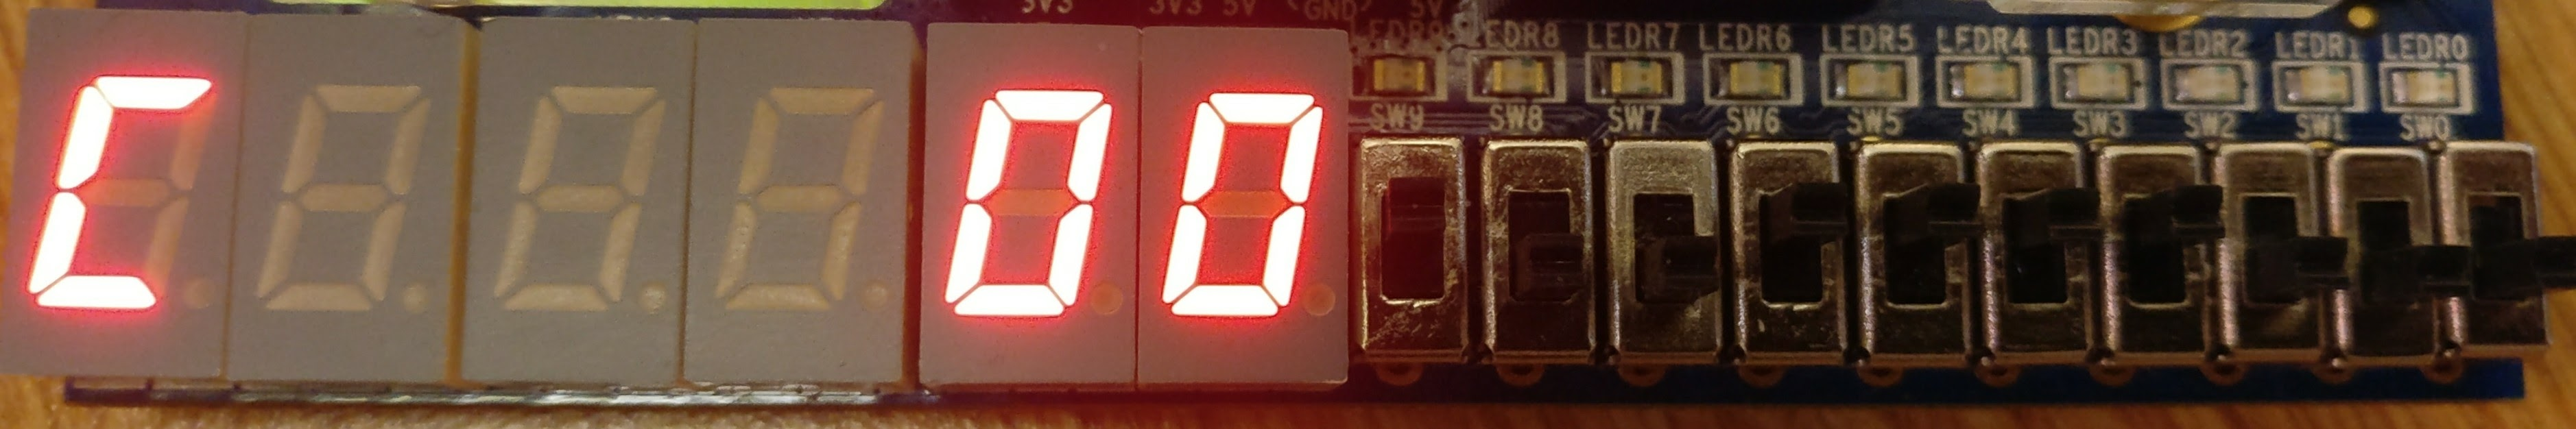
\includegraphics[width=0.8\textwidth]{C3}
    \caption{Our output for seeing if 0x8 is less than 0x7, showing that it is not.}
\end{figure}
\begin{figure}[H]
    \centering
    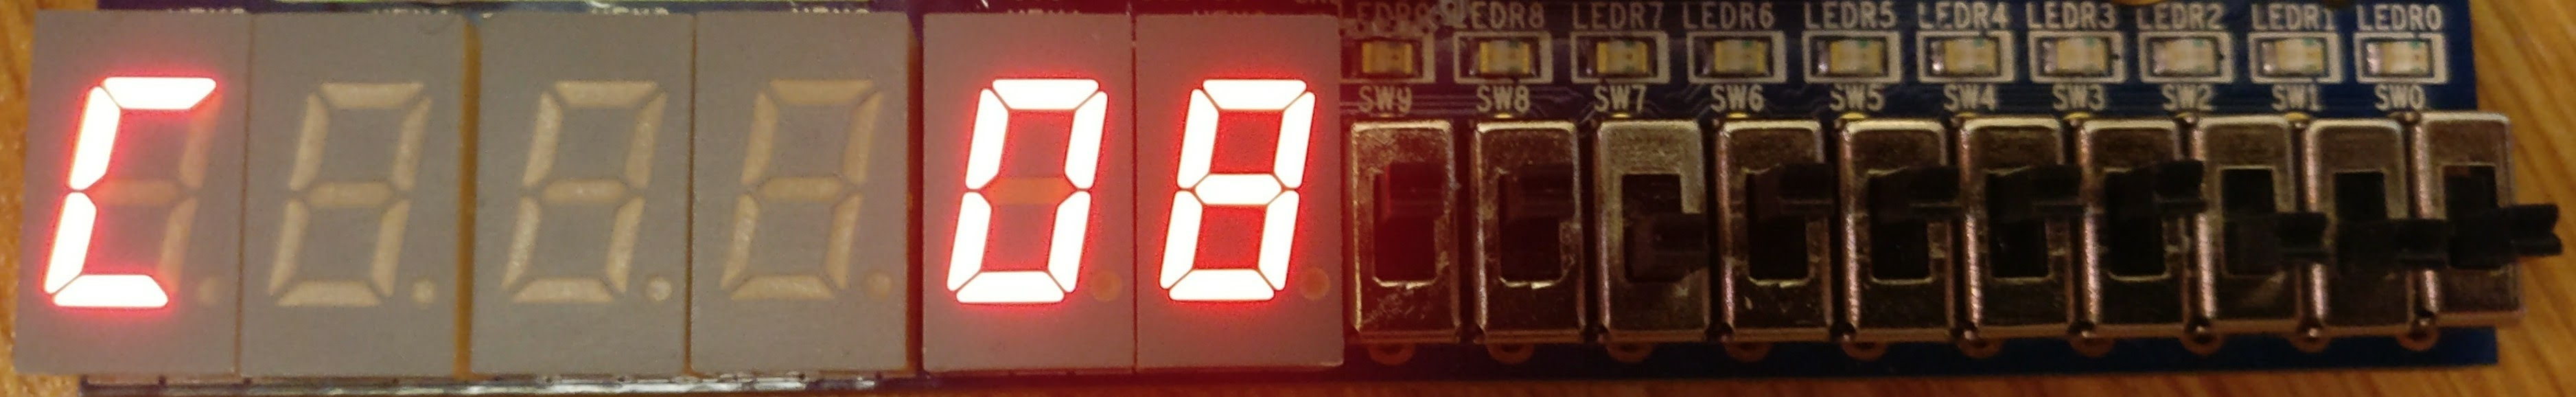
\includegraphics[width=0.8\textwidth]{C4}
    \caption{Our output for returning the max of 0x8 and 0x7, showing that it is 0x8.}
\end{figure}

\begin{figure}[H]
    \centering
    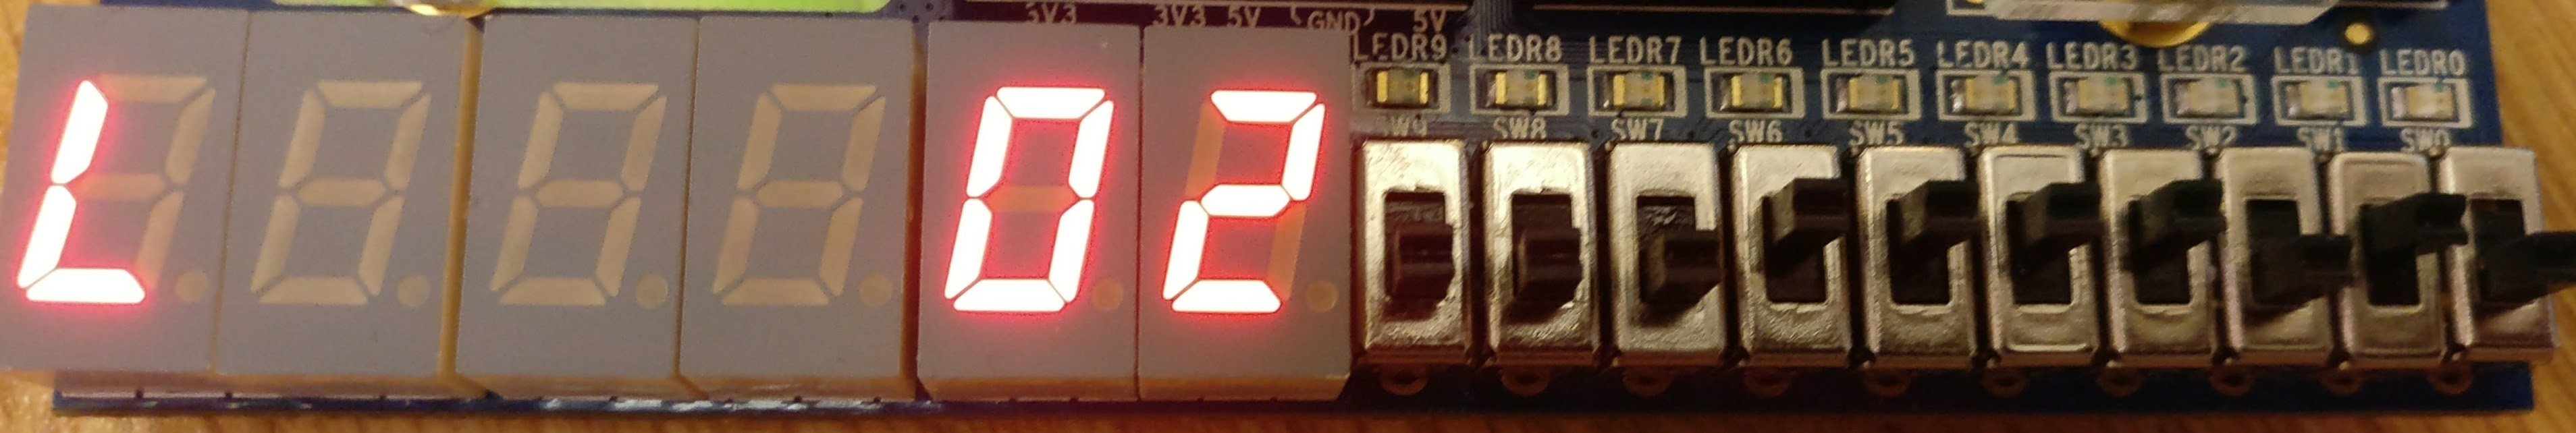
\includegraphics[width=0.8\textwidth]{L1}
    \caption{Our output for the bitwise and of 0xA and 0x7, showing that it is 0x2}
\end{figure}
\begin{figure}[H]
    \centering
    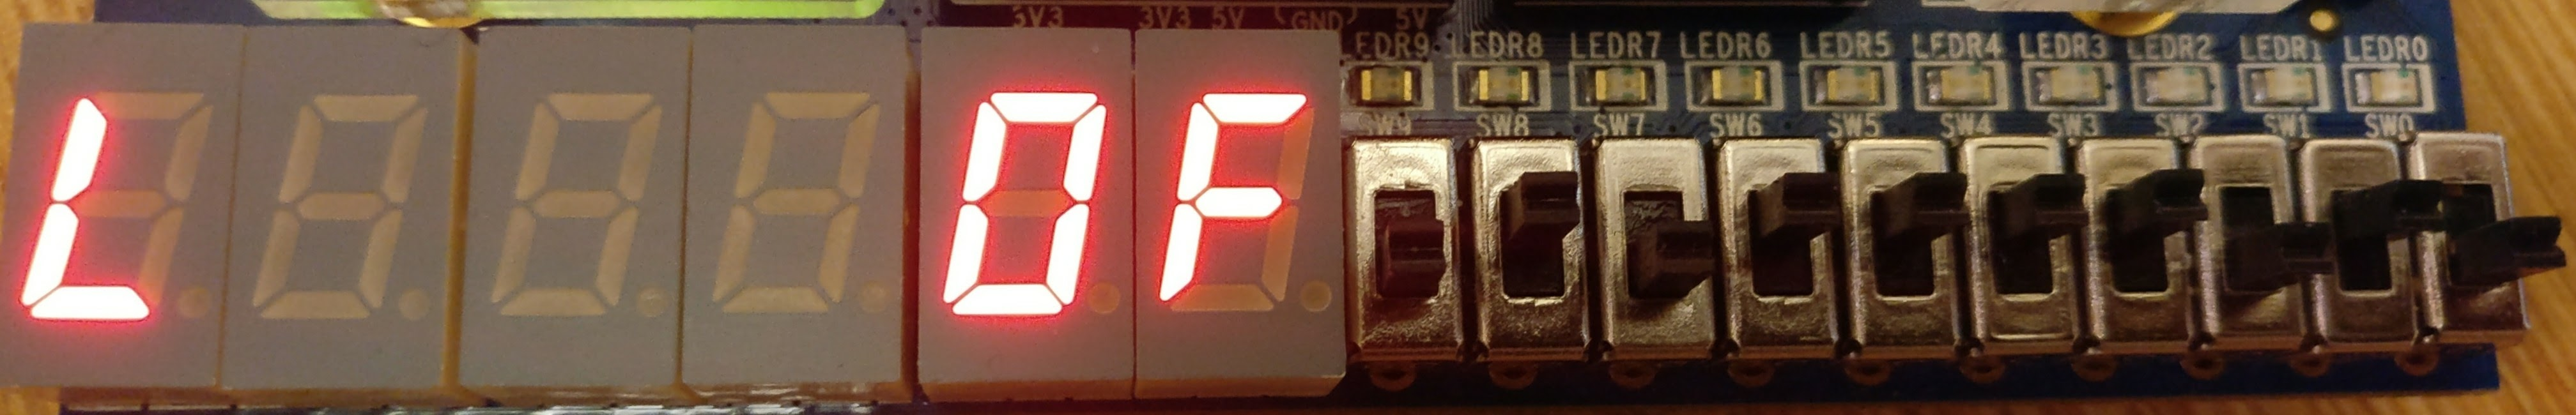
\includegraphics[width=0.8\textwidth]{L2}
    \caption{Our output for the bitwise or of 0xA and 0x7, showing that it is 0xF}
\end{figure}
\begin{figure}[H]
    \centering
    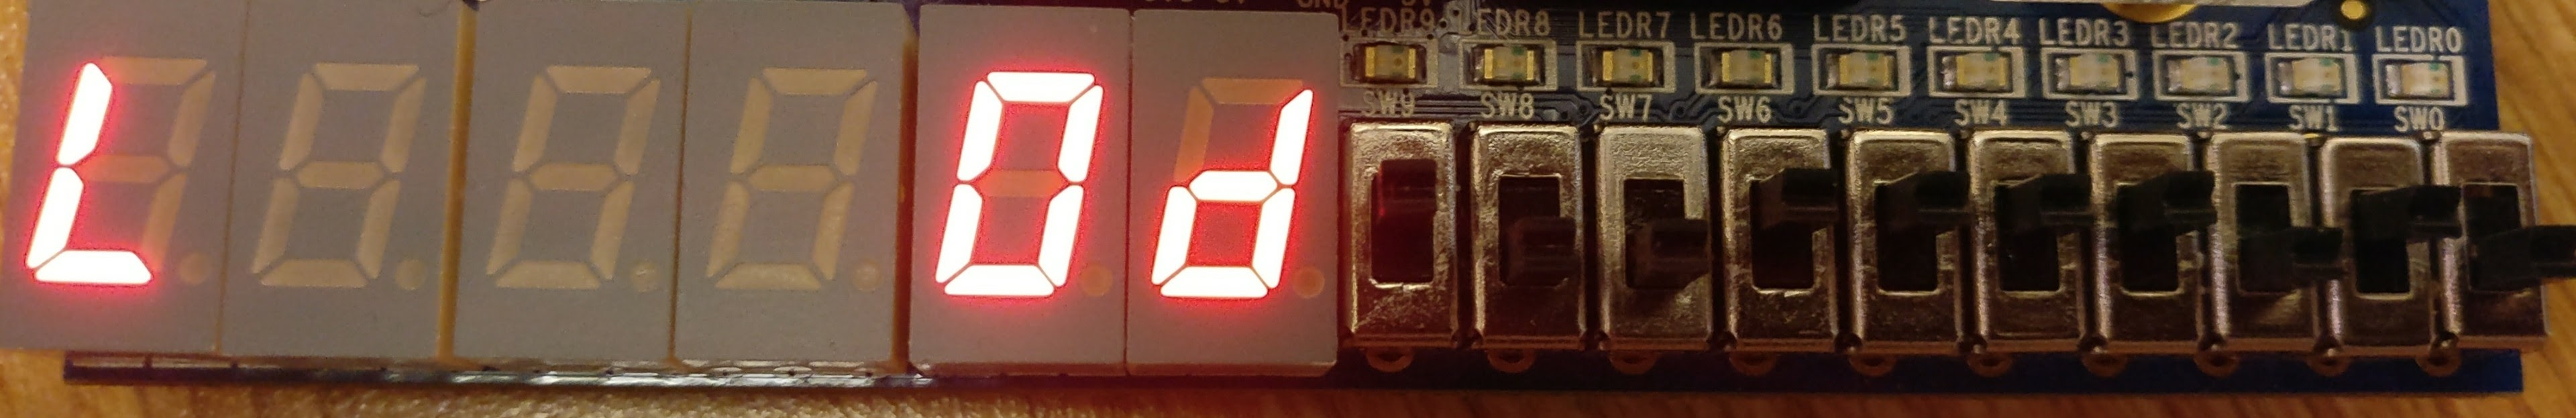
\includegraphics[width=0.8\textwidth]{L3}
    \caption{Our output for the bitwise exclusive or of 0xA and 0x7, showing that it is 0xd}
\end{figure}
\begin{figure}[H]
    \centering
    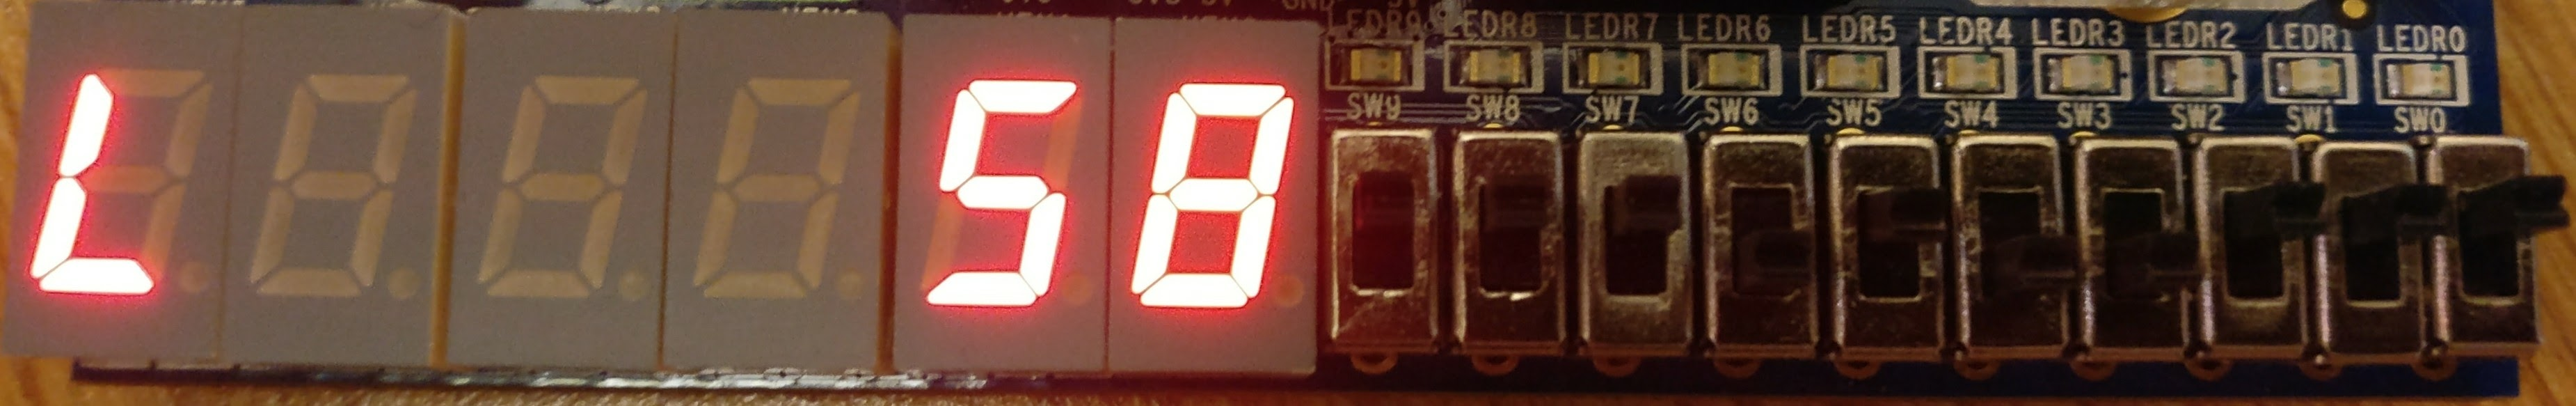
\includegraphics[width=0.8\textwidth]{L4}
    \caption{Our output for the bitwise not of 0xA7, showing that it is 0x53}
\end{figure}



\section{Conclusions}
This project was quite challenging in that we had no previous exposure to writing Verilog, using Quartus, or even necessarily having developed a solid intuition for digital design. An important part of the intuition we ended up developing was the idea that information is always being updated. We as a team struggled in that our default intuition is related to high level languages. It didn't matter if we pumped the switches into the code before we'd set a mode because they would be constantly updating anyway. However, this was a very good introductory project to expose us to a lot of really fascinating and useful functions. Displaying the generated block diagrams and exploring through them was quite satisfying and proved to solidify some of the concepts. The biggest bug we ran into was in making Magic. While it does work, in our time limit we were not able to move away from higher level thinking. Thus, magic is highly inefficient and ``hacky'', to quote Professor Fosdick. If given more time, we would redo magic to more explicitly take into account the system we are programming for. In general, we did not run into any glaring error or bugs that we could not resolve. The largest error that we worked on were syntax related. For example, the code written on the board during class had a couple very significant syntax errors. The order given in class read input/output, variable name, and then size. However, as it turns out, it actually is really important that size comes before the variable names.



\section{Conceptual Block Diagrams Appendix}
\begin{figure}[H]
    \centering
    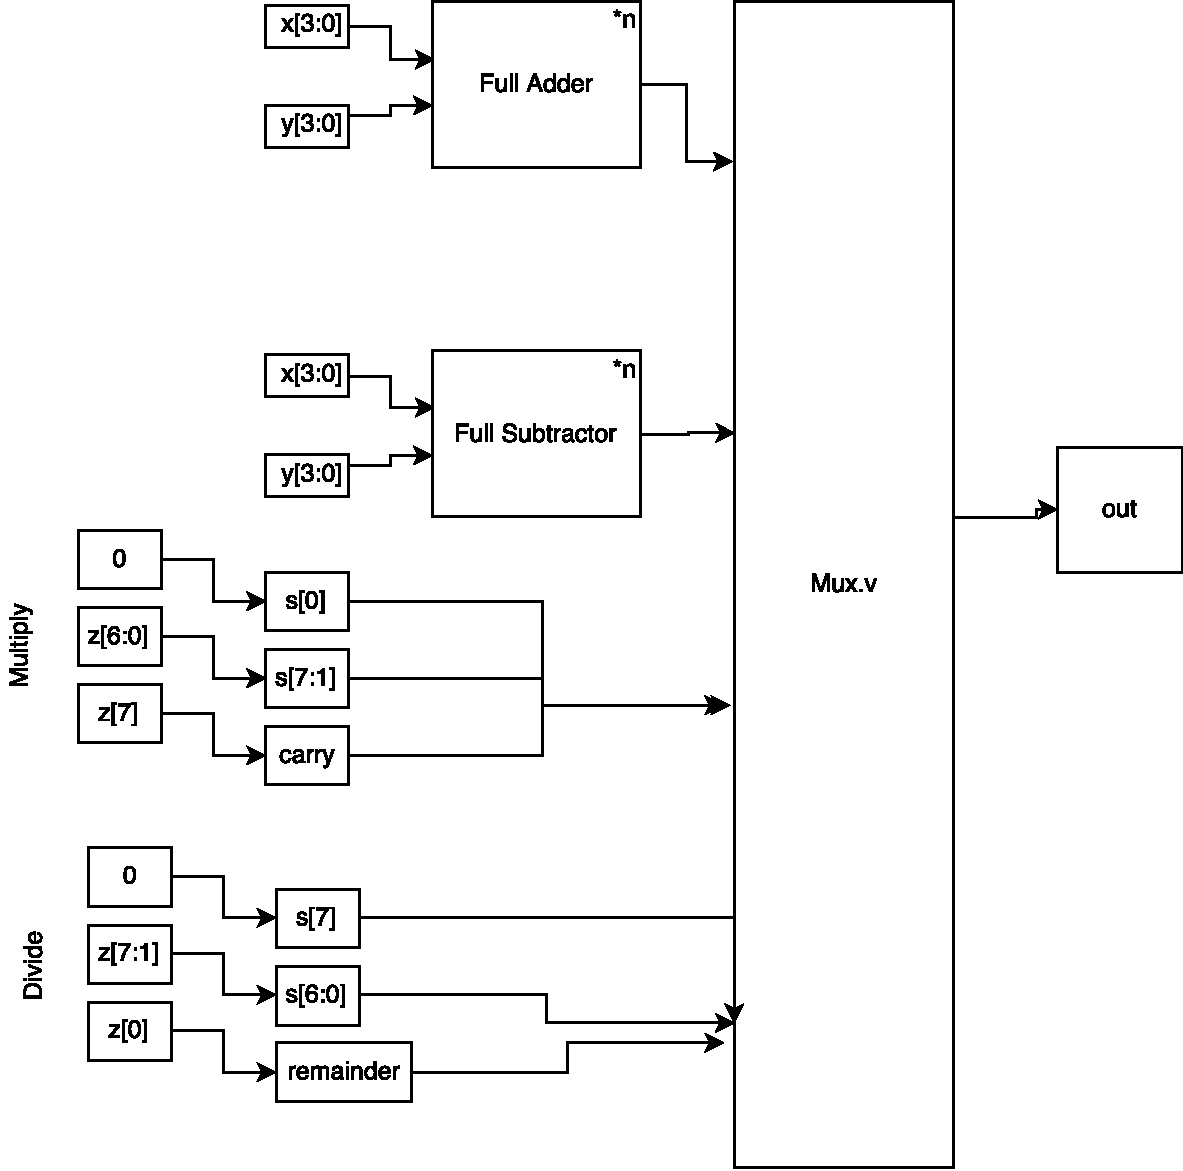
\includegraphics[clip, trim=0cm 0cm 0cm 0cm, width=0.8\textwidth]{Arithmetic_BD.pdf}
    \caption{Block Diagram of Arithmetic Mode}
    \label{fig:arithmeticdrawn}
\end{figure}

\begin{figure}[H]
    \centering
    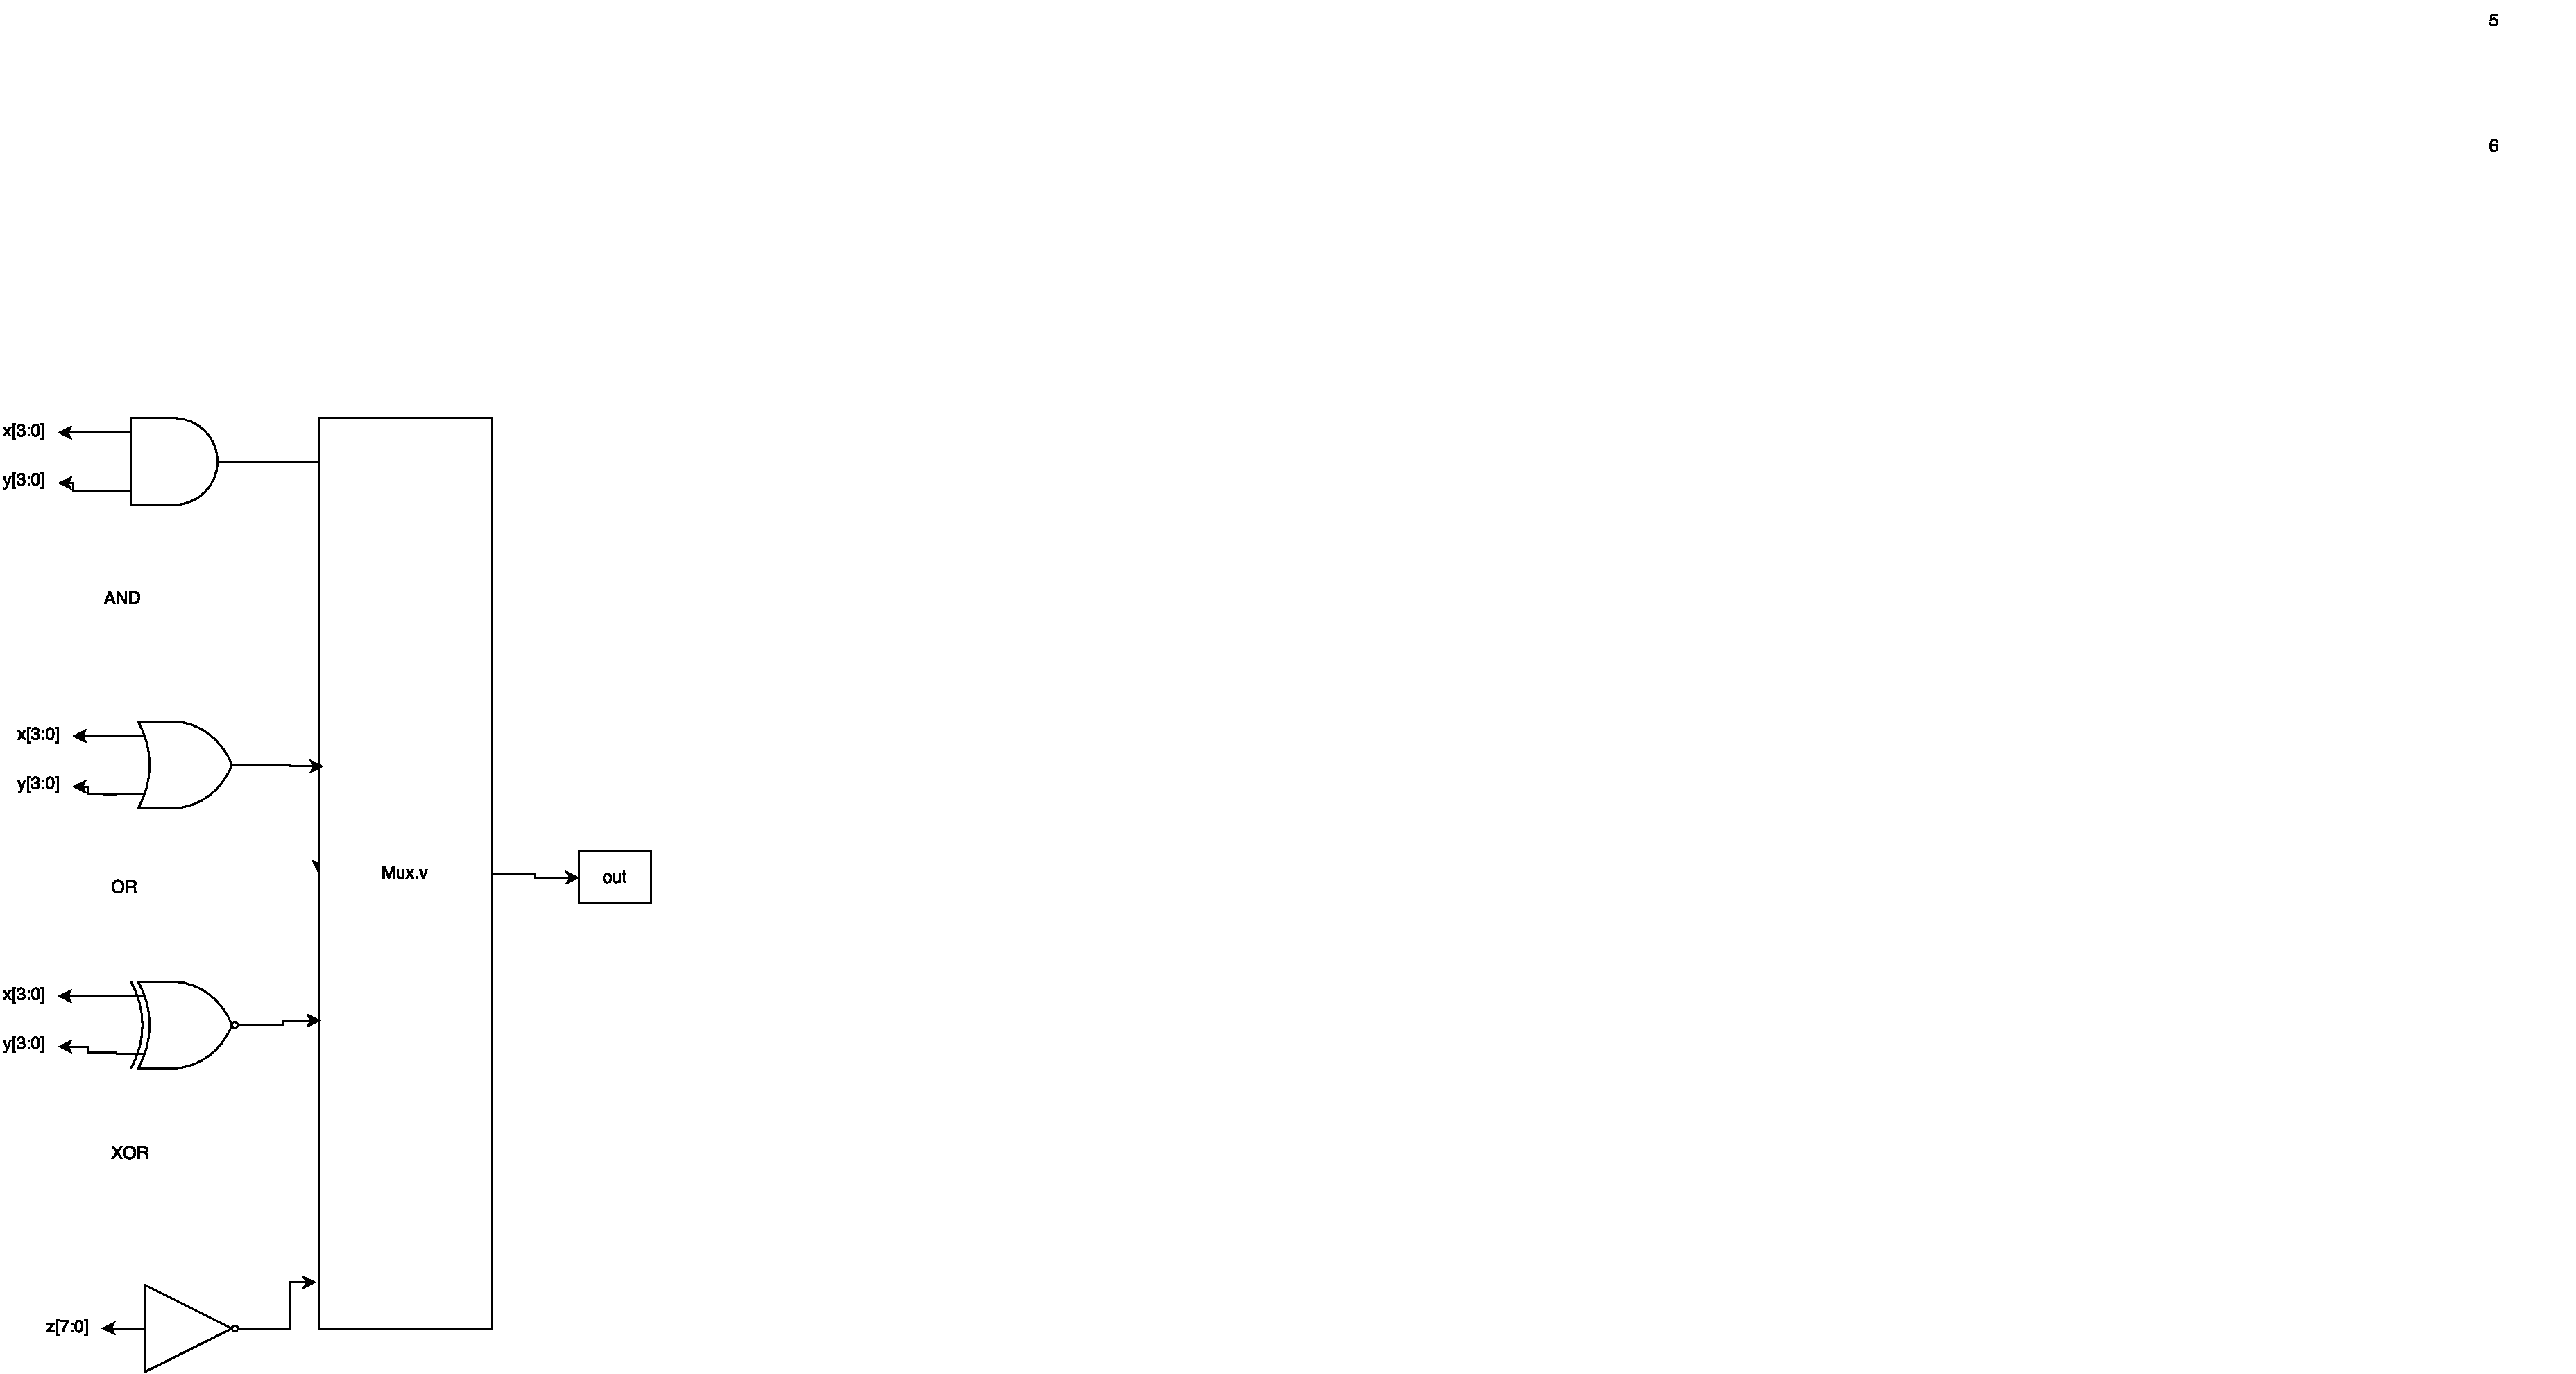
\includegraphics[clip, trim=0cm 0cm 45cm 10cm, width=0.8\textwidth]{Logical_BD.pdf}
    \caption{Block Diagram of Logical Mode}
    \label{fig:logicaldrawn}
\end{figure}

\begin{figure}[H]
    \centering
    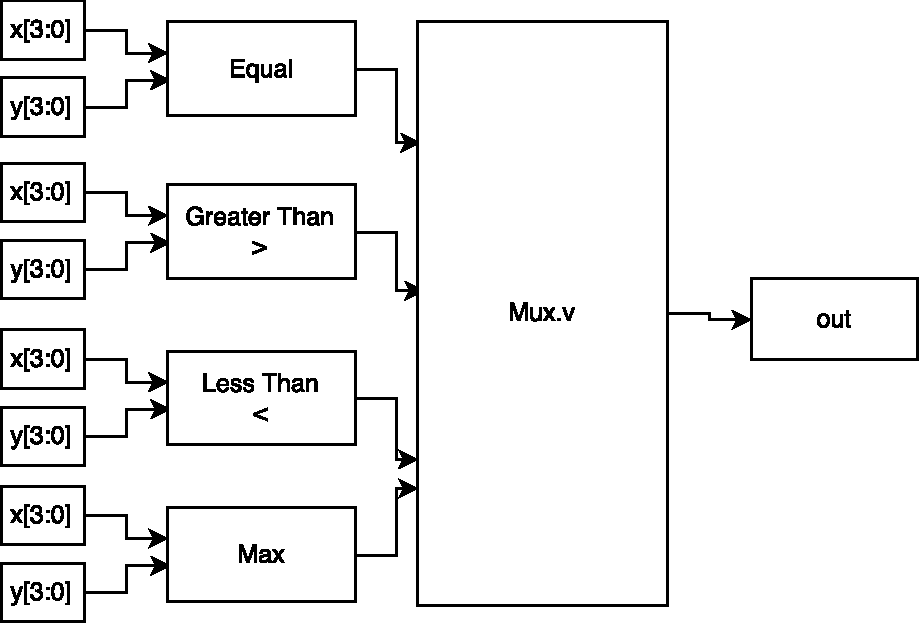
\includegraphics[clip, width=0.8\textwidth]{Comparison_BD.pdf}
    \caption{Block Diagram of Comparison Mode}
    \label{fig:comparisondrawn}
\end{figure}

\section{Generated Block Diagrams Appendix}
\begin{figure}[H]
    \centering
        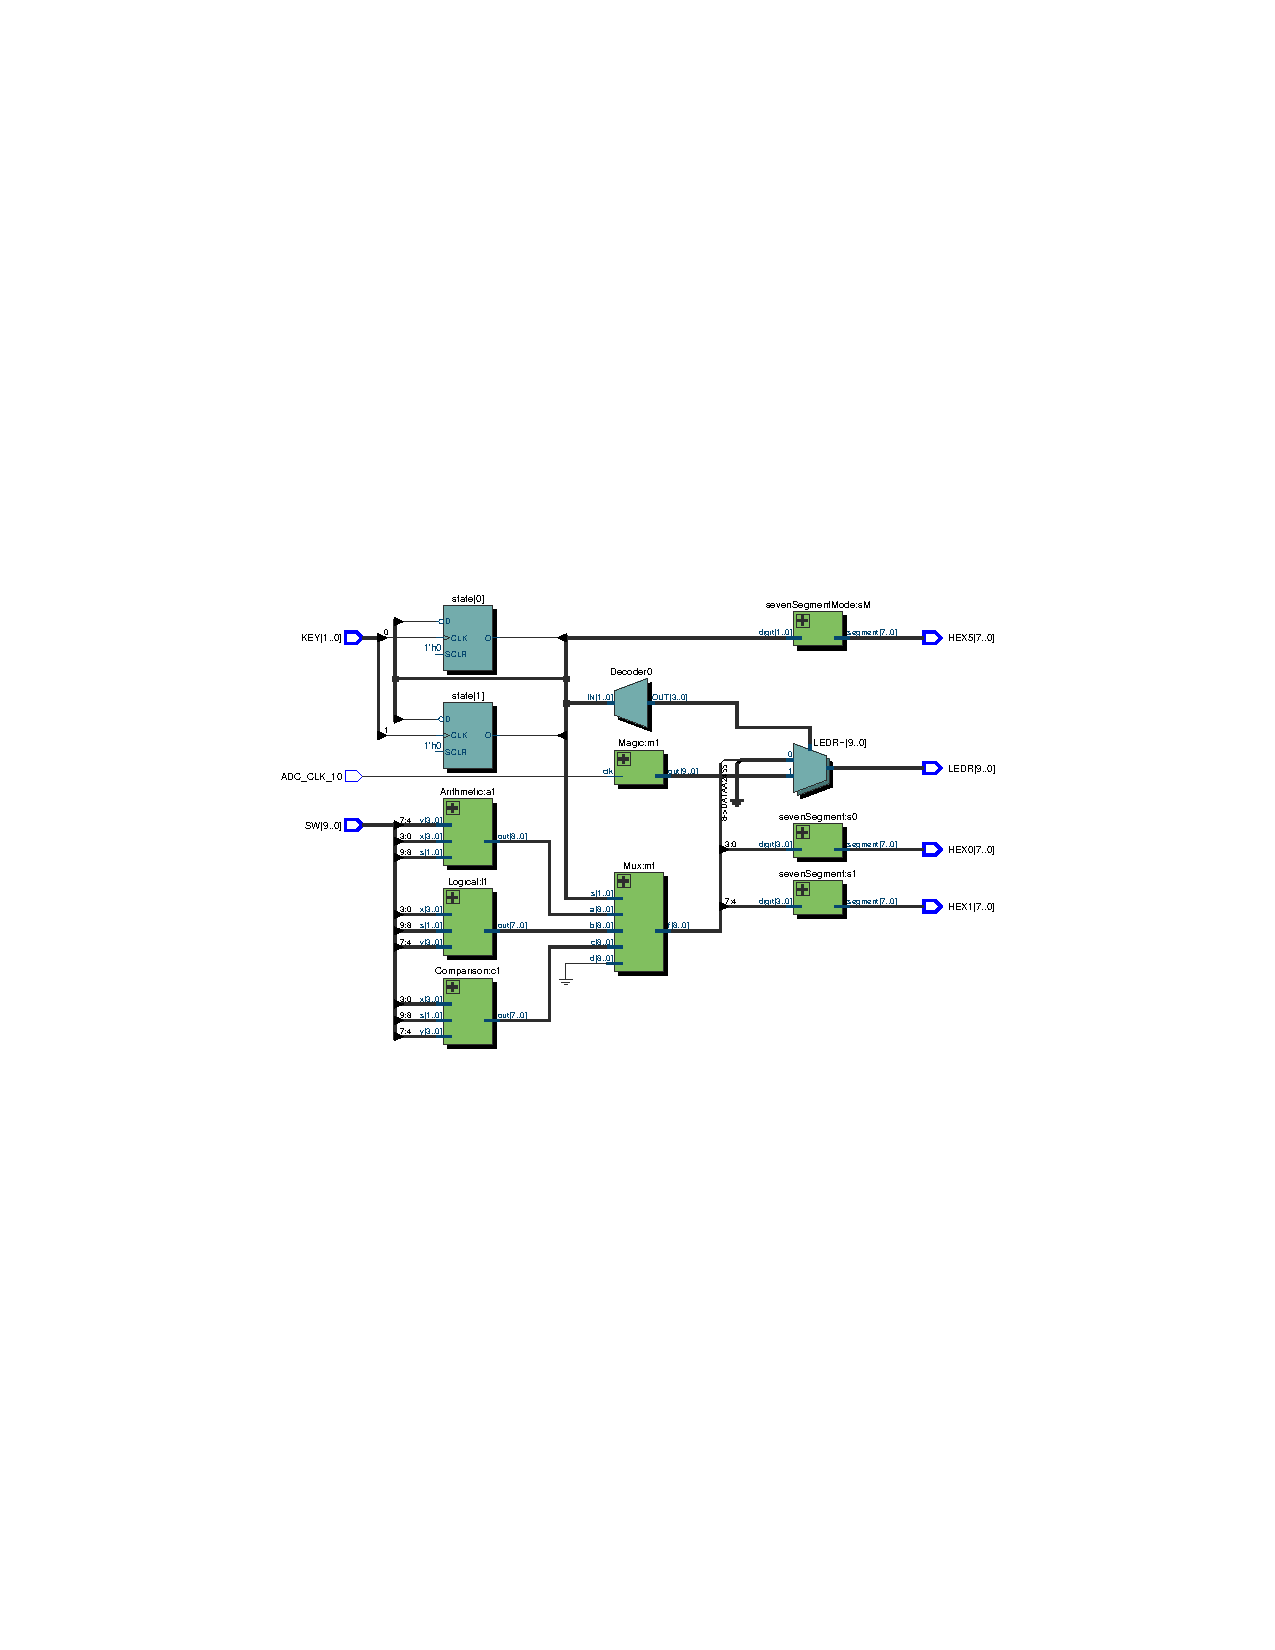
\includegraphics[clip, trim=3cm 10cm 3cm 10cm, width=\textwidth]{Top}
        \caption{Generated Block Diagram of our Top.v}
\end{figure}

\begin{figure}[H]
    \centering
        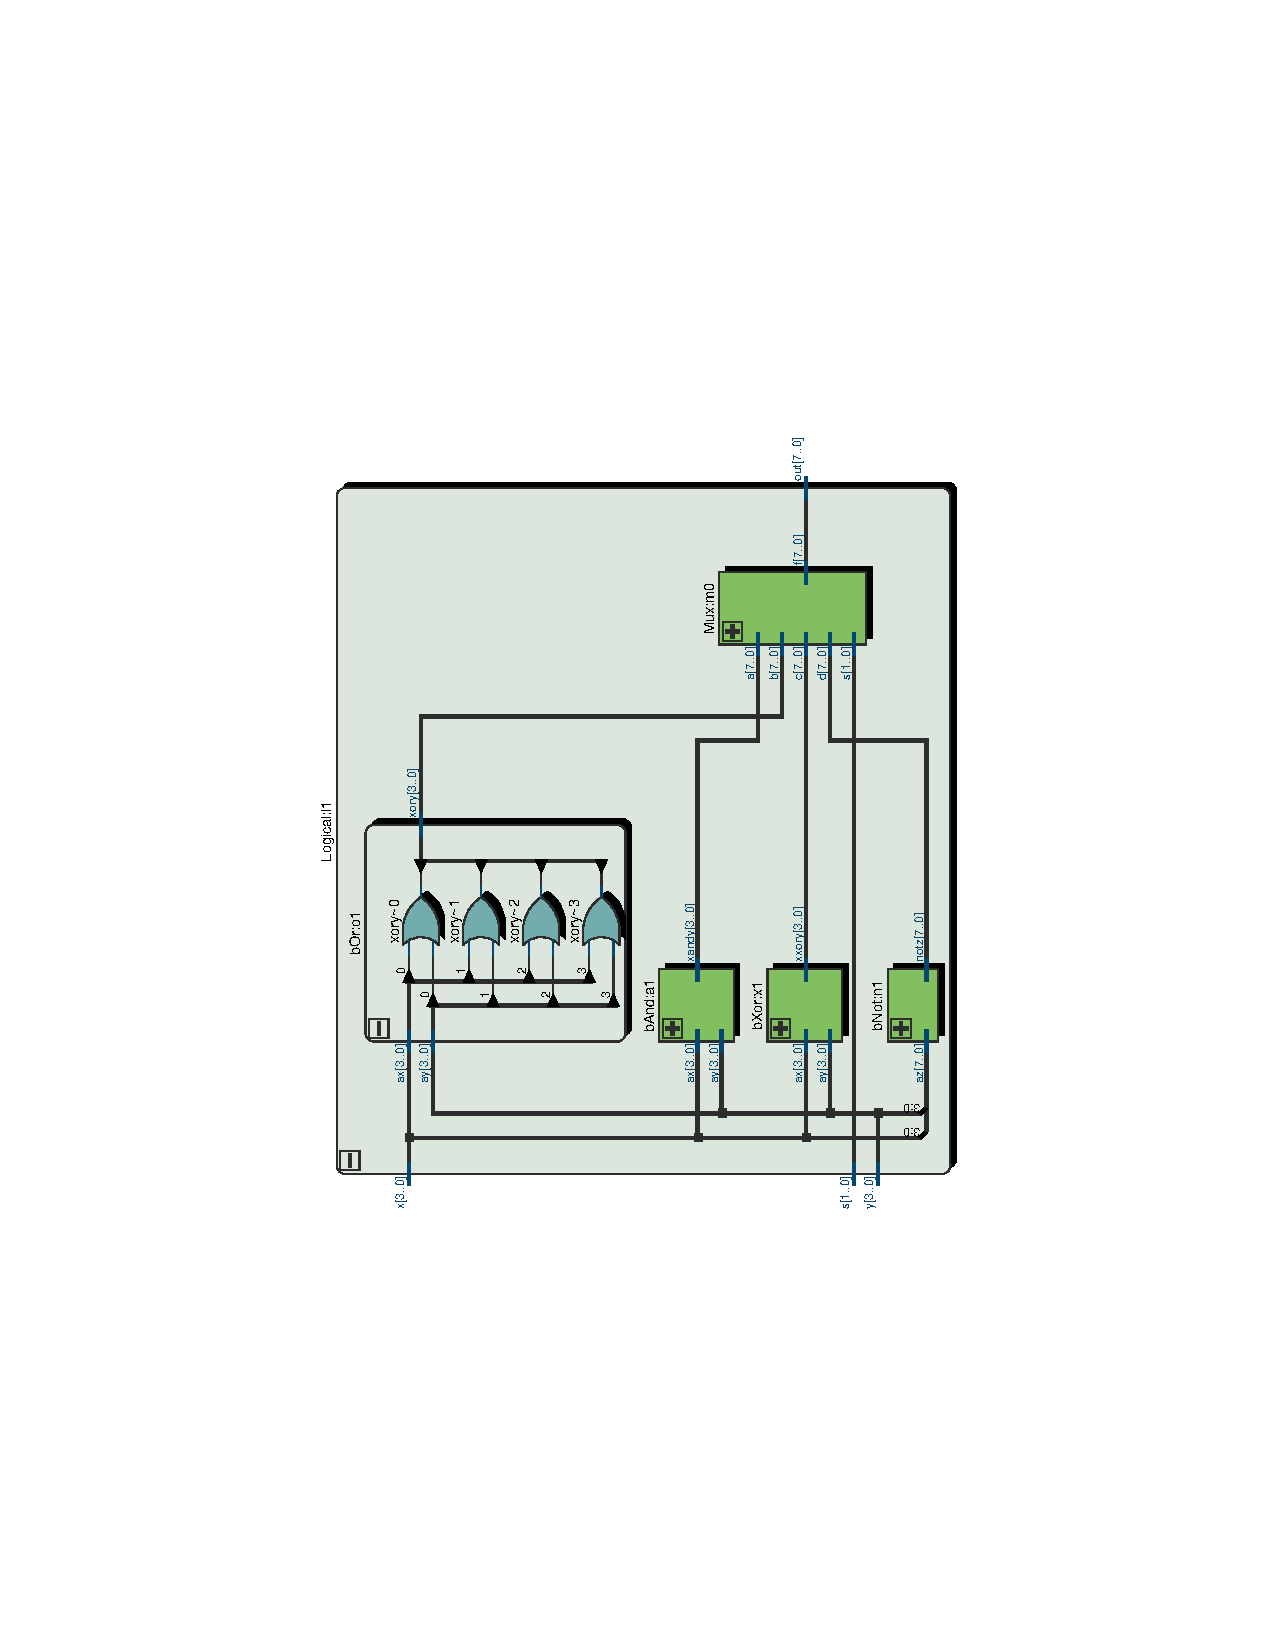
\includegraphics[clip, trim=5cm 6cm 5cm 6cm, angle=270, width=\textwidth]{Logical}
        \caption{Generated Block Diagram of our Logical.v, with our `or' module expanded as an example of how the other modules are laid out internally. }
    \label{fig:logicalgen}
\end{figure}

\begin{figure}[H]
    \centering
        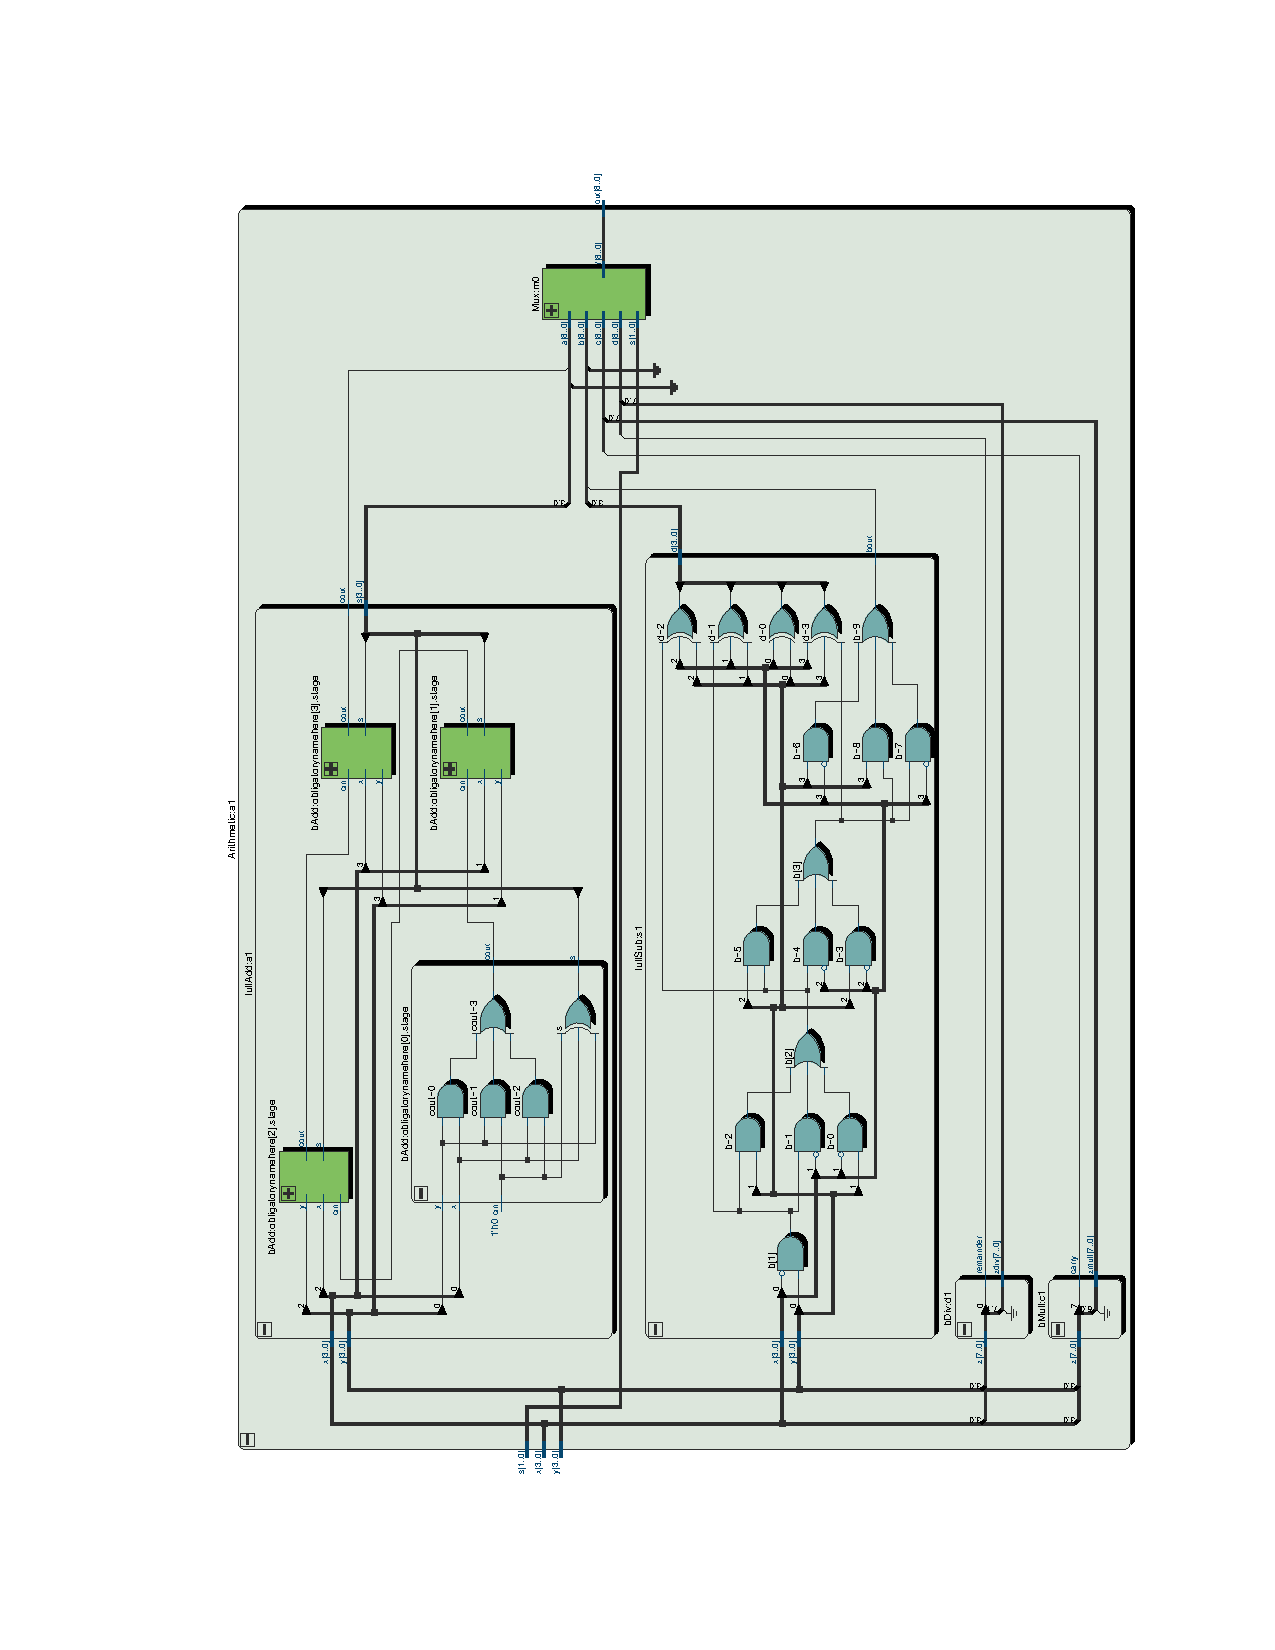
\includegraphics[clip, trim=3cm 3cm 2cm 3cm, angle=270,  width=\textwidth]{Arithmetic}
        \caption{Generated Block Diagram of our Arithmetic.v, showing the 4 bit adder with one module expanded and the full 4 bit subtractor.}
    \label{fig:arithmeticgen}
\end{figure}

\begin{figure}[H]
    \centering
        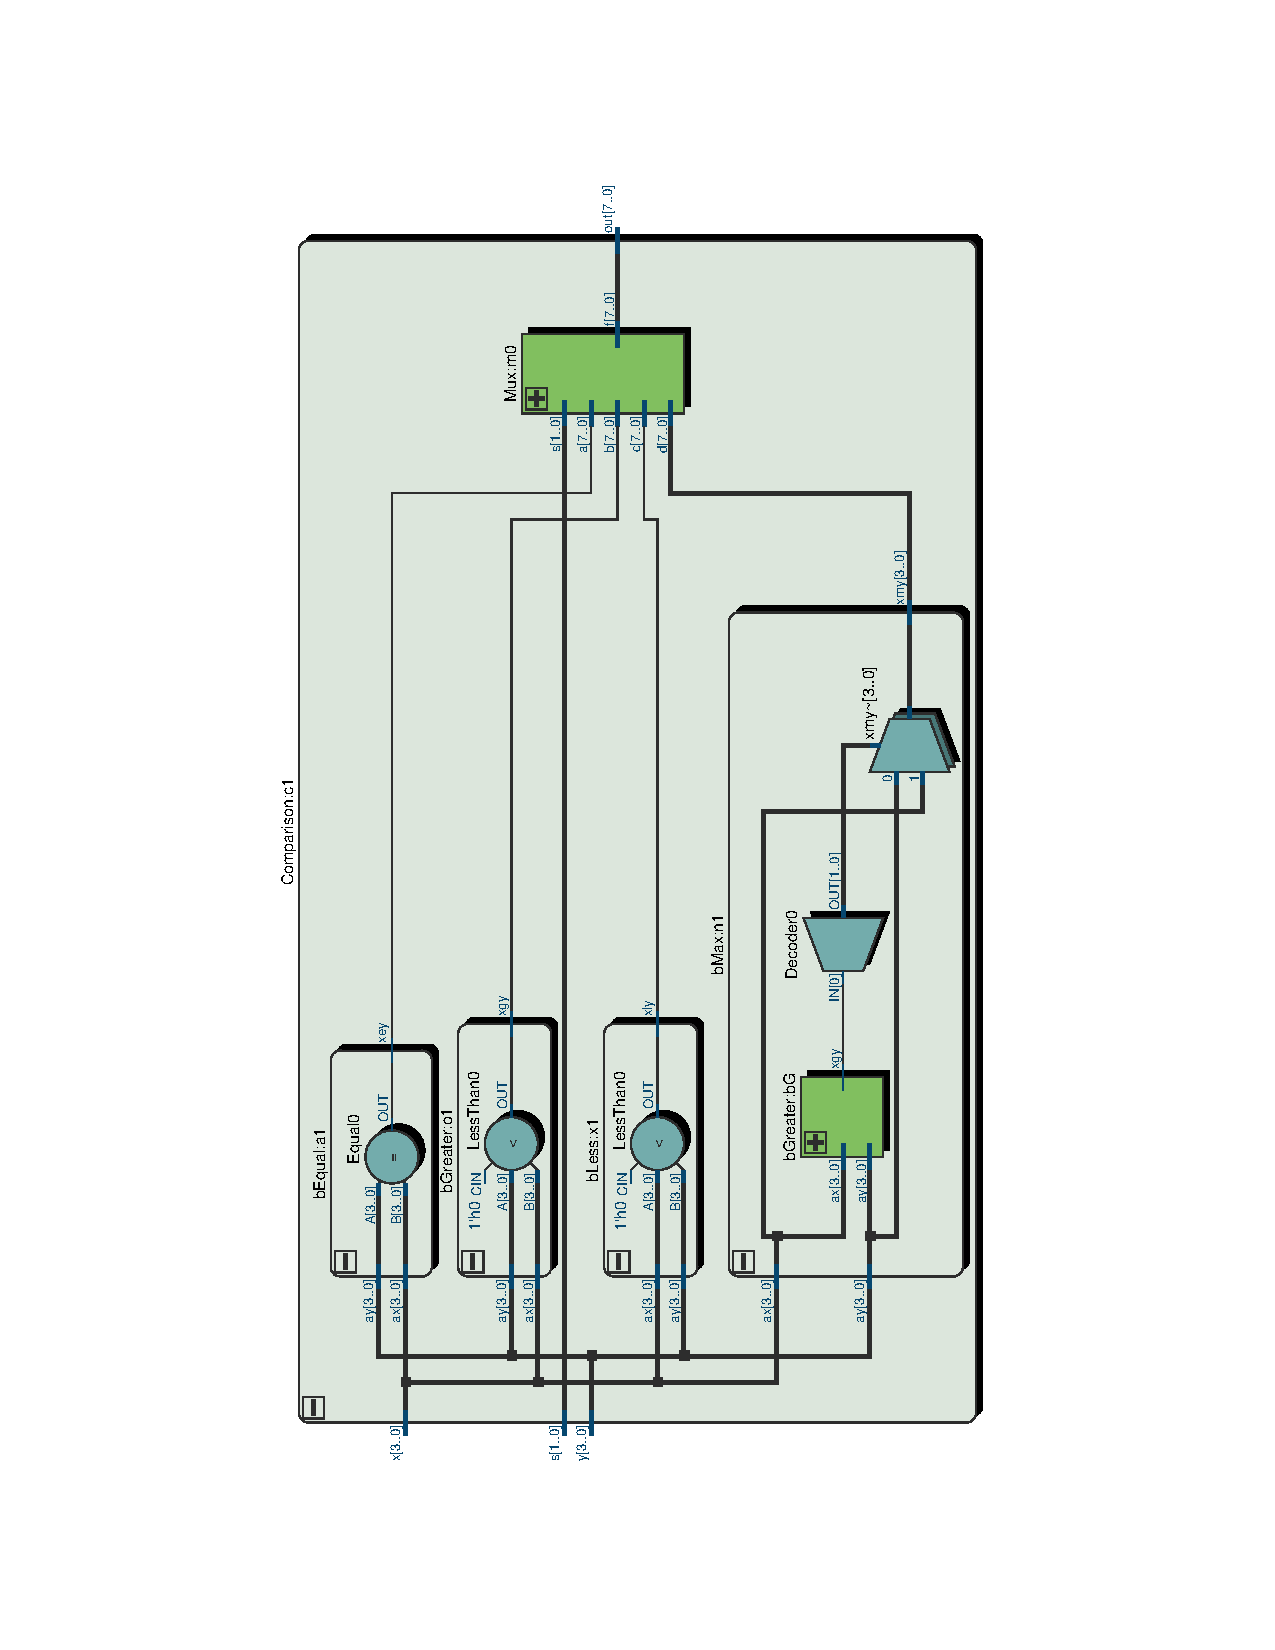
\includegraphics[clip, trim=4cm 3cm 5cm 3cm, angle=270,  width=\textwidth]{Comparison}
        \caption{Generated Block Diagram of our Comparison.v, with Max expanded to show its use of bGreater.}
    \label{fig:comparisongen}
\end{figure}

\begin{figure}[H]
    \centering
        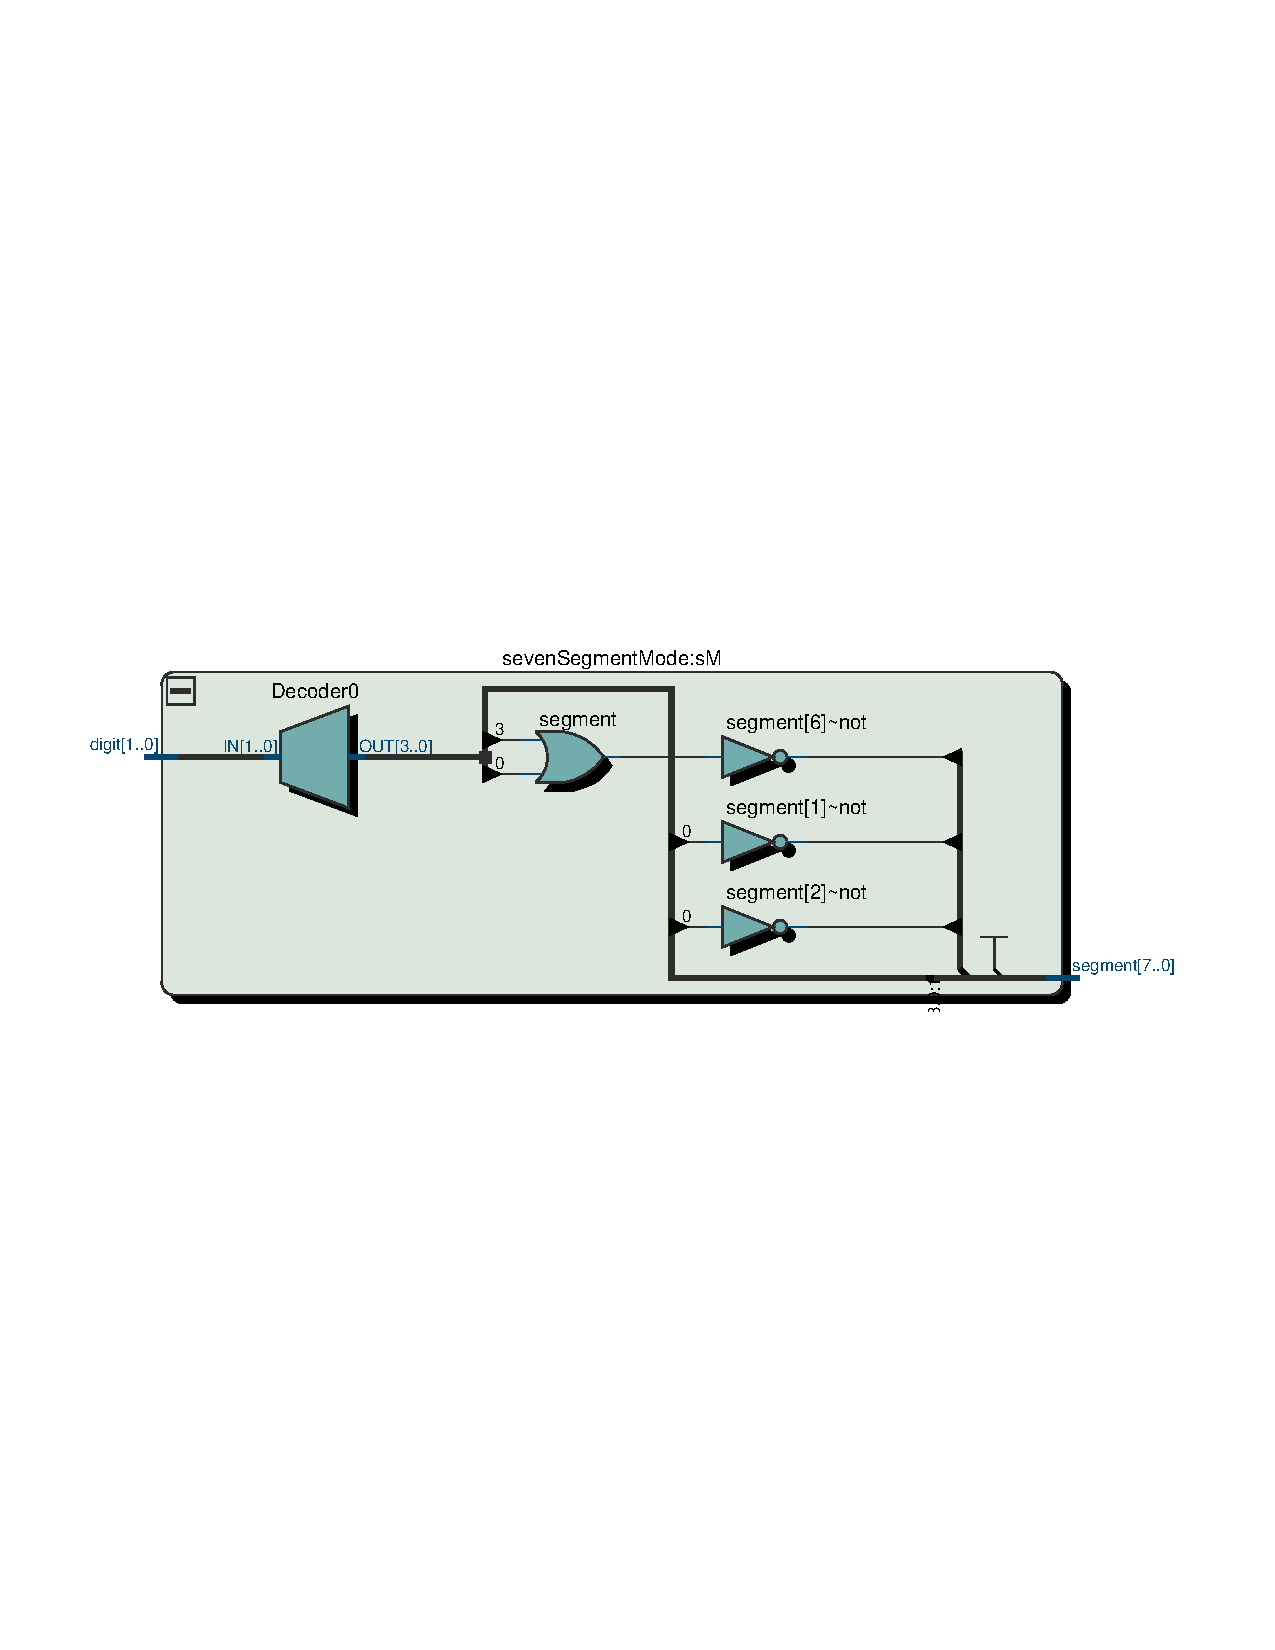
\includegraphics[clip, trim=0cm 9cm 0cm 9cm,  width=\textwidth]{SevenSegmentMode}
        \caption{Generated Block Diagram of our SevenSegmentMode.v, showing how Quartus compiled our always/case statments for the mode indicator.}
\end{figure}

\begin{figure}[H]
    \centering
        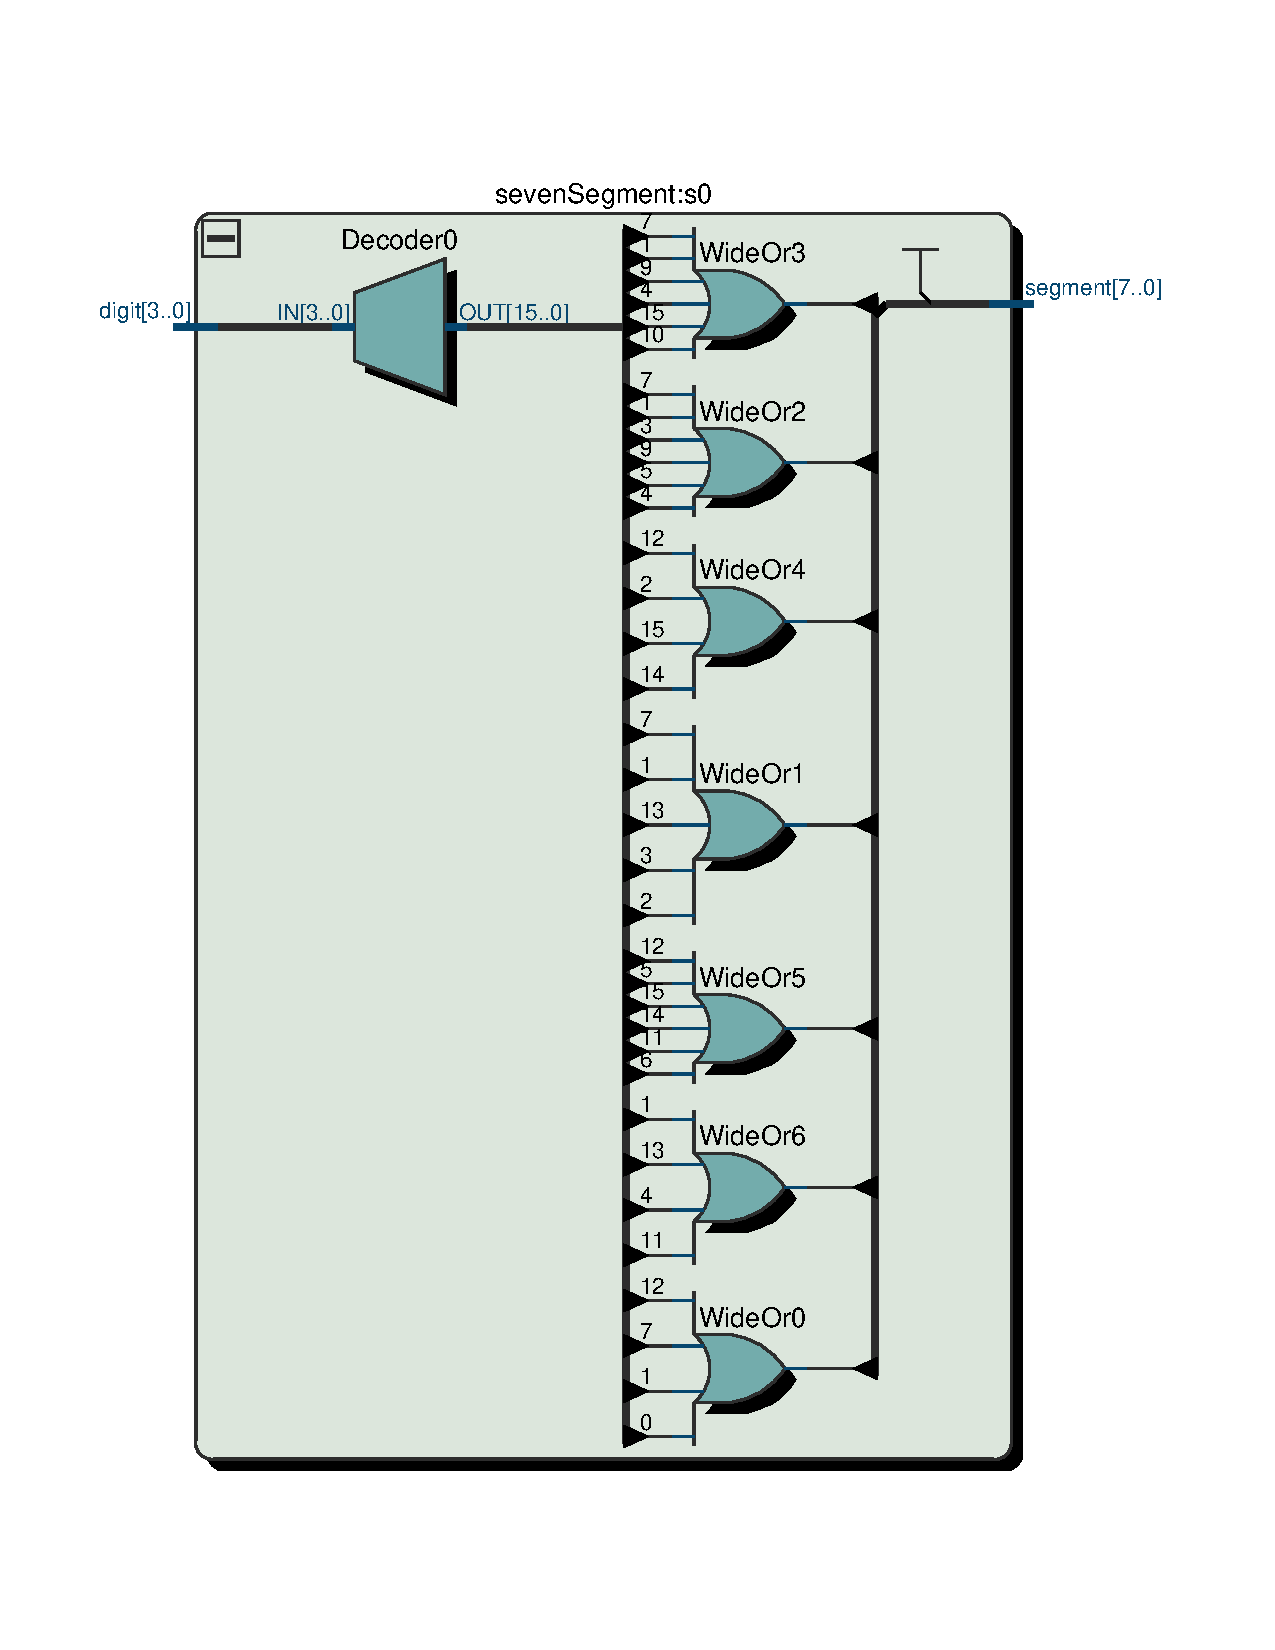
\includegraphics[clip, trim=0cm 3cm 0cm 3cm,  width=\textwidth]{SevenSegment}
        \caption{Generated Block Diagram of our SevenSegment.v, showing how Quartus compiled our always/case statments.}
\end{figure}

\begin{figure}[H]
    \centering
        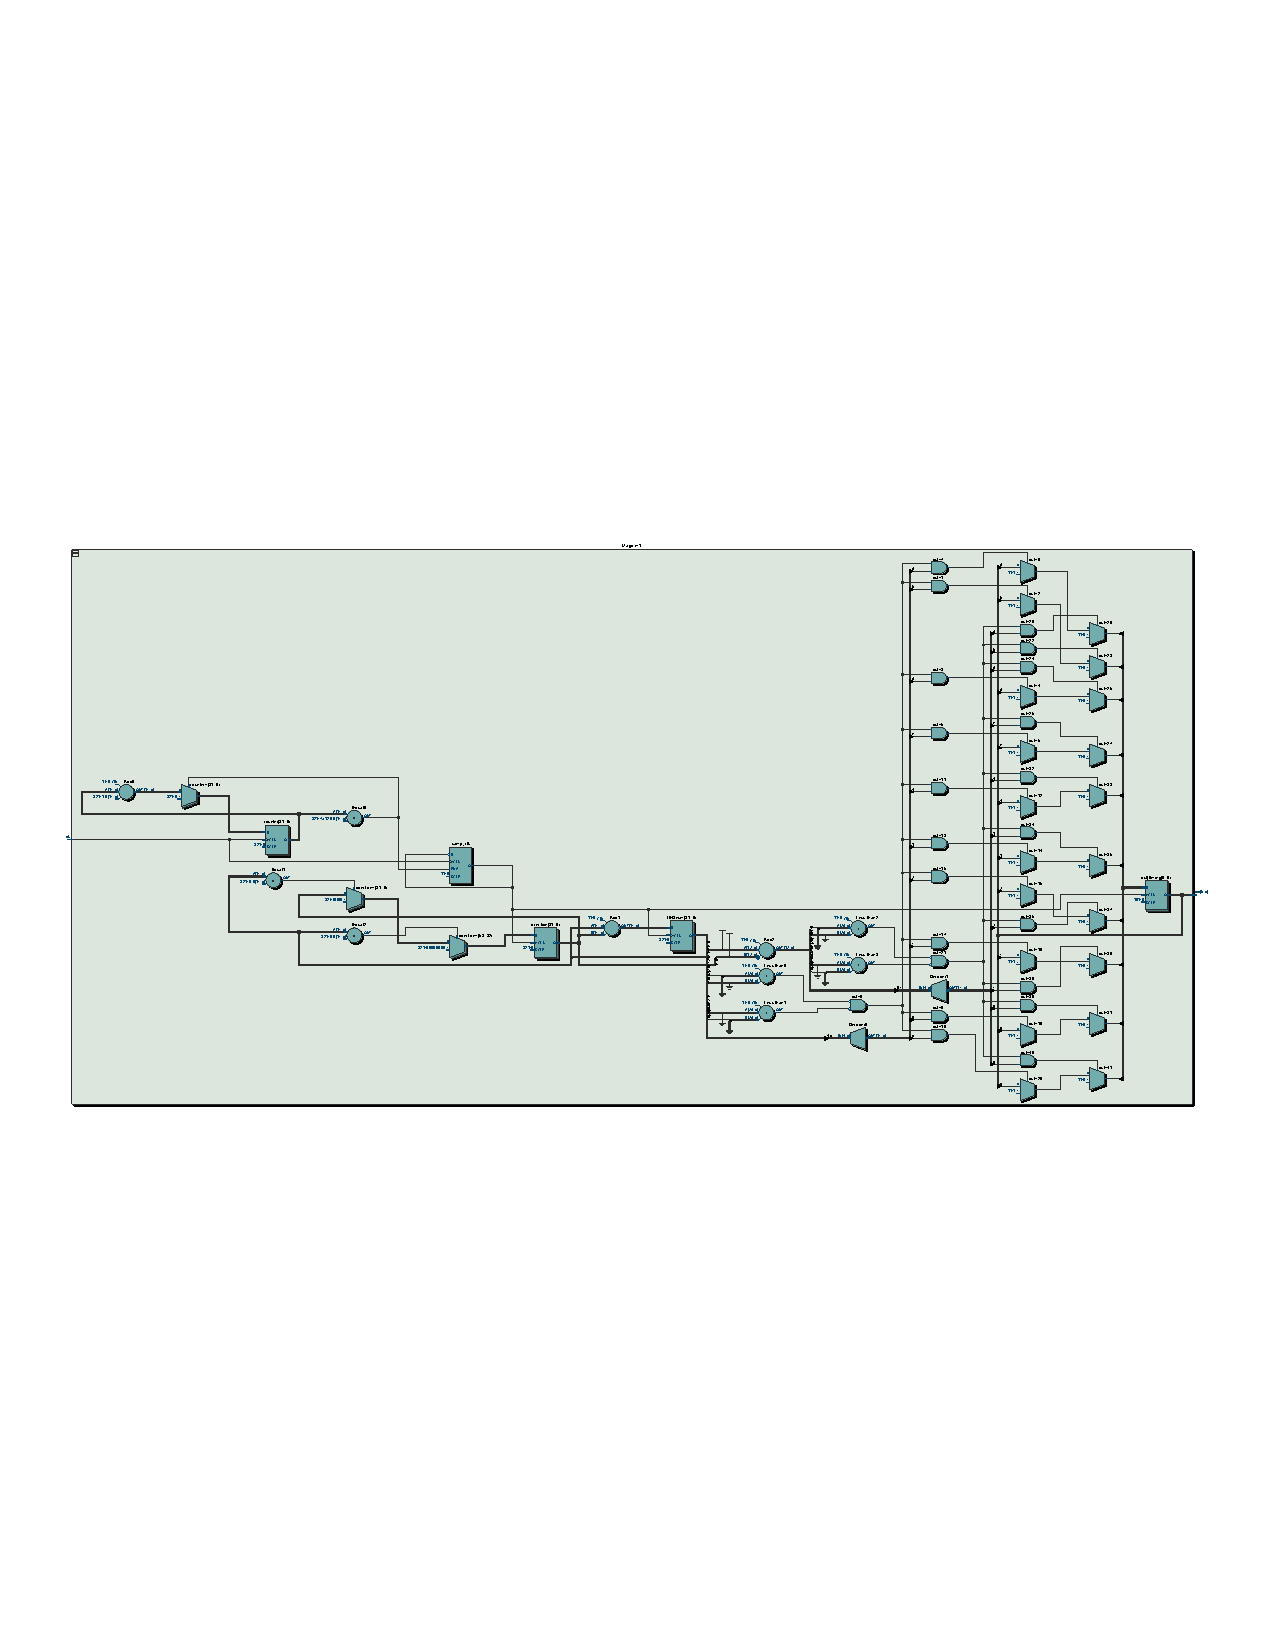
\includegraphics[clip, trim=1cm 9cm 1cm 7cm,  width=\textwidth]{Magic}
        \caption{Generated Block Diagram of our Magic.v, showing how Quartus compiled our always/case statements and integer arithmetic from some very C-esqe code down into a very inefficient gate setup.}
\end{figure}


\end{document}
